
%\documentclass[10pt,a4paper]{article}
\documentclass[runningheads]{llncs}

\usepackage[utf8]{inputenc}
\usepackage{amsmath,amsfonts,amssymb}
\usepackage{thmtools}
%\usepackage{amsthm}
\usepackage{thm-restate}

\usepackage{hyperref}
\usepackage[capitalize, noabbrev]{cleveref}
\usepackage{graphicx}
\usepackage{color}
\usepackage{enumerate}
\usepackage{caption}
\usepackage{subcaption}
\usepackage{array}
\usepackage{authblk}

\usepackage{tikz,tikzsymbols}
\usetikzlibrary{shapes,patterns,positioning}
\usetikzlibrary{arrows,decorations.markings}
\usetikzlibrary{calc}

                  
%%%%%%%%%%%%%%%%%%%%%%%%%%%%%%%%%%%%%%%%%%%%%%
%%  Macros
%%%%%%%%%%%%%%%%%%%%%%%%%%%%%%%%%%%%%%%%%%%%%%
\newcommand{\RR}{\mathbb{R}}
\newcommand{\NN}{\mathbb{N}}
\newcommand{\ZZ}{\mathbb{Z}}

\newcommand{\set}[1]{\{ #1 \}}
\newcommand{\fromto}[2]{\set{#1, \ldots, #2}}
\newcommand{\bigO}{\mathcal{O}}
\newcommand{\dotunion}{\mathbin{\dot{\cup}}}

\newcommand{\comment}[1]{\textcolor{red}{(L: #1)}}

\newcommand{\xxxNTP}{{\sc N-TreePack}}
\newcommand{\xxxHAM}{{\sc Hamilton-3-reg}}
\DeclareMathOperator{\ntp}{\text{\sf ntp}}
\newcommand{\greedy}{\text{\sf Greedy}}

\newcommand{\lasse}[1]{\textcolor{blue}{#1}}



%%%%%%%%%%%%%%%%%%%%%%%%%%%%%%%%%%%%%%%%%%%%%%%%%%%%%%%%%%%%%%%%%%%%%%%%%%
%%%%%%%%%%%%%%%%%%%%%%%%%%%%%%%%%%%%%%%%%%%%%%%%%%%%%%%%%%%%%%%%%%%%%%%%%%
%%%%%%%%%%%%%%%%%%%%%%%%%%%%%%%%%%%%%%%%%%%%%%%%%%%%%%%%%%%%%%%%%%%%%%%%%%
%%%%%%%%%%%%%%%%%%%%%%%%%%%%%%%%%%%%%%%%%%%%%%%%%%%%%%%%%%%%%%%%%%%%%%%%%%
\sloppy
\begin{document}

\title{Non-preemptive tree packing}
\titlerunning{Non-preemptive tree packing}

\author{Stefan Lendl\inst{1} \and
Gerhard Woeginger\inst{2} \and
Lasse Wulf\inst{3,*}
}

\authorrunning{S. Lendl, G. Woeginger, and L. Wulf}
\institute{Department of Operations and Information Systems, University of Graz, Austria 
%\email{stefan.lendl@uni-graz.at}\\
\and Department of Computer Science, RWTH Aachen, Germany 
%\email{woeginger@algo.rwth-aachen.de}\\
\and Institute of Discrete Mathematics, Graz University of Technology, Austria\\ 
*Corresponding author: \email{wulf@math.tugraz.at}
}
%
\maketitle 

\begin{abstract}
An instance of the non-preemptive tree packing problem consists of an undirected graph $G=(V,E)$ 
together with a weight $w(e)$ for every edge $e\in E$.
The goal is to activate every edge $e$ for some time interval of length $w(e)$, such that the 
activated edges keep $G$ connected for the longest possible overall time.

We derive a variety of results on this problem.
The problem is strongly NP-hard even on graphs of treewidth~$2$, and it does not allow a polynomial
time approximation scheme (unless P=NP).
Furthermore, we discuss the performance of a simple greedy algorithm, and we construct and analyze
a number of parameterized and exact algorithms.
\end{abstract}


%%%%%%%%%%%%%%%%%%%%%%%%%%%%%%%%%%%%%%%%%%%%%%%%%%%%%%%%%%%%%%%%%%%%%%%%%
%%%%%%%%%%%%%%%%%%%%%%%%%%%%%%%%%%%%%%%%%%%%%%%%%%%%%%%%%%%%%%%%%%%%%%%%%
\section{Introduction}
%%%%%%%%%%%%%%%%%%%%%%%%%%%%%%%%%%%%%%%%%%%%%%%%%%%%%%%%%%%%%%%%%%%%%%%%
\paragraph{The tree packing problem of Nash-Williams.}
For a given undirected connected graph $G=(V,E)$ and a weight function $w:E\to\NN$,
Nash-Williams \cite{Nash-Williams1961} considered \lasse{the optimization problem of packing as many spanning trees as possible into the graph, such that for every edge $e \in E$, it gets used in at most $w(e)$ spanning trees. For example, consider \cref{fig_spt_example}, where $G$ is a complete grap on three vertices, and $w(e) = 2$ for all edges. The optimal solution packs three spanning trees. It is not possible to pack more spanning trees, because every edge already is used twice.} 
%%%%%%%%%%%%%%%%%%%%%%%
\begin{figure}[htpb]
\centering
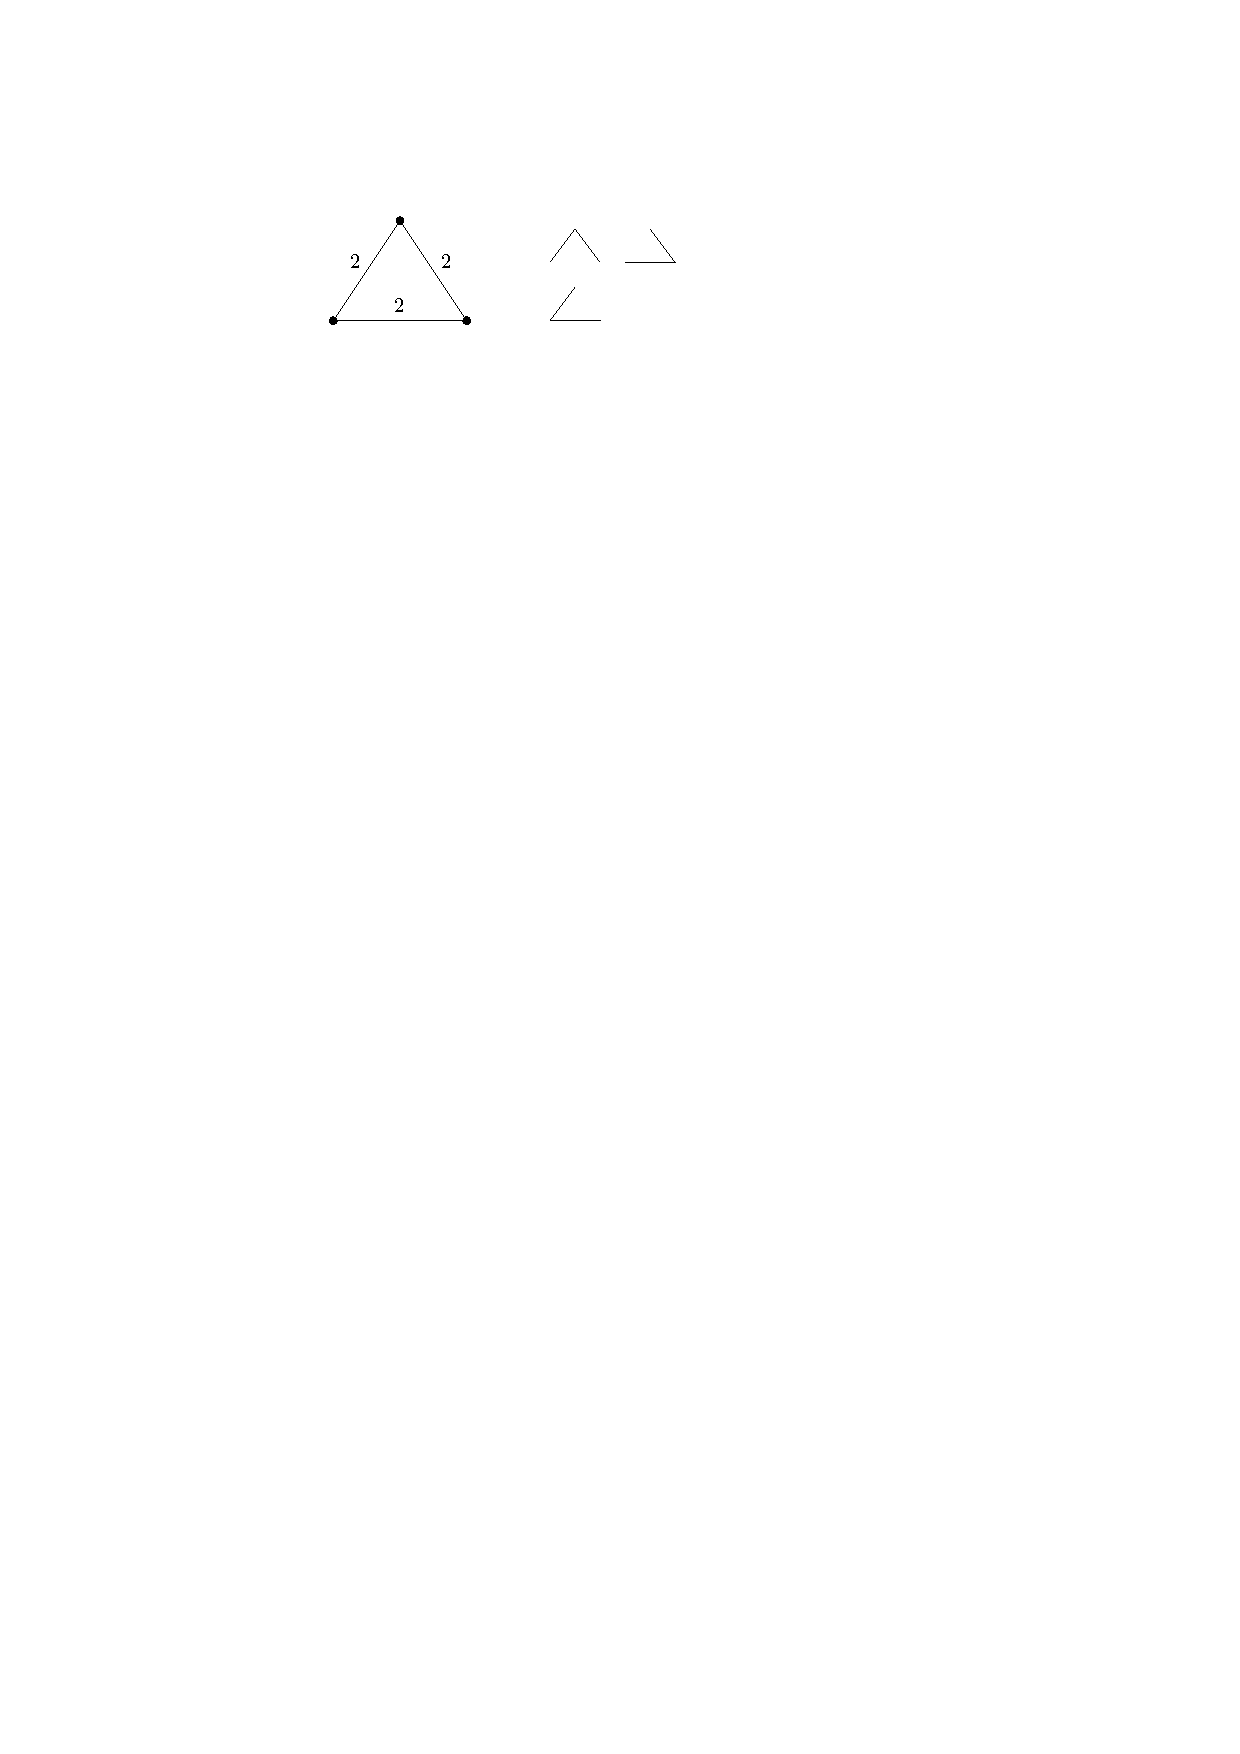
\includegraphics[scale=1]{img/stp-example}
\caption{\lasse{An instance of Nash-Williams spanning tree packing problem. The optimal solution packs three spanning trees, as indicated on the right.}}
\label{fig_spt_example}
\end{figure}
%%%%%%%%%%%%%%%%%%%%%%%
Nash-Williams \cite{Nash-Williams1961} derives a min-max relation for the problem that connects it to certain cut conditions.
Building on these results, Cunningham \cite{Cunningham1985} constructs a polynomial time 
algorithm for the problem by reducing it to a polynomial number of maximum flow problems.
Barahona \cite{Barahona1995} presents another algorithm with a better time complexity.

the tree packing problem may also be interpreted as a scheduling problem:
Every edge $e\in E$ is a resource that can be activated for a total of $w(e)$ time units.
The objective now is to activate the edges in such a way that the graph remains connected 
for the longest possible overall time. 
%Under this interpretation, the variable $x_T$ indicates the number of time units in which
%the spanning tree $T$ is used in the activation schedule.
Figure~\ref{fig:example} contains a simple illustrating example on the three-vertex cycle.
There are three spanning trees (that each consist of two edges), and an optimal schedule 
uses each of these spanning trees for exactly one time unit.
It is easy to see that in every optimal schedule, one of the three edges will be active 
during the first and the third time slot and will be inactive during the second time slot;
in the language of scheduling, we say that the execution of that edge is preempted 
at time $1$ and afterwards resumed at time $2$.
(In the schedule shown in Figure~\ref{fig:example}, edge $e_3$ is the preempted edge.)

%%%%%%%%%%%%%%%%%%%%%%%%%%%%%%%%%%%%%%%%%
\begin{figure}[tbh]
\begin{center}
%%%%%%%%%%%%%%%%
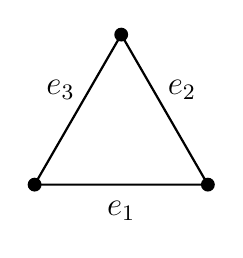
\begin{tikzpicture}[scale=1.10]
\coordinate (p1) at (-1,0);
\coordinate (p2) at ( 1,0);
\coordinate (p3) at ( 0,1.732);

\foreach \x in {1,2,3} \fill (p\x) circle (0.08);
\draw[thick] (p1)--(p2)--(p3)--(p1);
\node[] at  ( 0.0,-0.3) {\large $e_1$};
\node[] at  ( 0.7, 1.1) {\large $e_2$};
\node[] at  (-0.7, 1.1) {\large $e_3$};
\end{tikzpicture}
%%%%%%%%%%%%%%%%
\qquad\qquad
%%%%%%%%%%%%%%%%
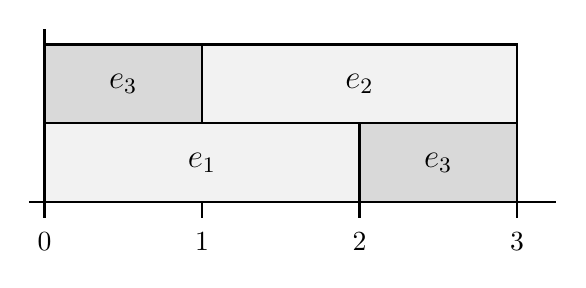
\begin{tikzpicture}[scale=1.00]
\draw[thick] (-0.2,0)--(6.5,0);
\draw[thick] (0,-0.2)--(0,2.2);

\node[] at  (0,-0.5) {$0$};
\draw[thick] (2,-0.2)--(2,0);
\draw[thick] (4,-0.2)--(4,0);
\draw[thick] (6,-0.2)--(6,0);
\node[] at  (2,-0.5) {$1$};
\node[] at  (4,-0.5) {$2$};
\node[] at  (6,-0.5) {$3$};

\draw[fill=gray,fill opacity=0.1,draw=black,thick,text opacity=1.0]
       (0,0) rectangle (4,1) node[pos=.5] {\large $e_1$};
\draw[fill=gray,fill opacity=0.3,draw=black,thick,text opacity=1.0]
       (4,0) rectangle (6,1) node[pos=.5] {\large $e_3$};

\draw[fill=gray,fill opacity=0.3,draw=black,thick,text opacity=1.0]
       (0,1) rectangle (2,2) node[pos=.5] {\large $e_3$};
\draw[fill=gray,fill opacity=0.1,draw=black,thick,text opacity=1.0]
       (2,1) rectangle (6,2) node[pos=.5] {\large $e_2$};
\end{tikzpicture}
%%%%%%%%%%%%%%%%
\end{center}
\caption{The three edges in the graph on the left hand side have weights $w(e_1)=w(e_2)=w(e_3)=2$.
The schedule on the right hand side keeps the graph connected for a total of three time units.}
\label{fig:example}

\vspace{-0.8cm}
\end{figure}
%%%%%%%%%%%%%%%%%%%%%%%%%%%%%%%%%%%%%%%%%

%%%%%%%%%%%%%%%%%%%%%%%%%%%%%%%%%%%%%%%%%
\paragraph{The non-preemptive version of tree packing.}
We consider a non-preemptive variant of the above tree packing problem,
where the execution of edges must not be preempted: 
Every edge $e$ is activated at some time point $\tau(e)$ chosen by the scheduler, and then 
remains active without interruption during the full time interval $[\tau(e),\,\tau(e)+w(e)]$.
The objective is again to activate the edges in such a way that the graph
remains connected for the longest possible overall time.
The resulting combinatorial optimization problem is called \emph{non-preemptive tree packing}
({\xxxNTP} for short), and the optimal objective value for a graph $G=(V,E)$ with edge 
weights $w:E\to\NN_0$ will be denoted $\ntp(G,w)$.

In the example in Figure~\ref{fig:example}, every reasonable non-preemptive
schedule will either activate two of the edges at time~$0$, or activate the three
edges respectively at times $0,1,2$.
As there is no way of keeping the graph connected for more than two time units, 
the optimal objective value is $\ntp(G,w)=2$.

%%%%%%%%%%%%%%%%%%%%%%%%%%%%%%%%%%%%%%%%%
\paragraph{Contributions of this paper.}
We analyze the computational complexity and the approximability of non-preemptive 
tree packing, and we also provide some parameterized and exact algorithms for it.
The complexity results are devastating:
\begin{itemize}
\item {\xxxNTP} is strongly NP-hard, even on complete bipartite graphs $K_{2,n}$. 
\item {\xxxNTP} is strongly NP-hard, even on graphs of bandwidth~$2$.
\end{itemize}
\lasse{(A problem is \emph{strongly NP-hard} if it stays NP-hard even if all its numerical parameters are bounded by a polynomial.)} Since complete bipartite graphs $K_{2,n}$ are series-parallel and since graphs of 
bandwidth~$2$ are outerplanar, our results yield strong NP-hardness for essentially 
all natural subclasses of graphs with treewidth~$2$.
As edges of zero-weight are irrelevant for the objective value of {\xxxNTP}, NP-hardness 
immediately propagates from graphs to supergraphs; hence our results also imply 
strong NP-hardness for all the standard families of specially structured graphs, 
like planar graphs, bipartite graphs, interval graphs, cographs, etc.
The only notable exception are the trees and the cactus graphs.
Furthermore, we analyze the complexity of cases with small objective values:
Deciding whether $\ntp(G,w)\ge\beta$ can be done in polynomial time for $\beta=3$
and is NP-hard for $\beta=7$; the intermediate cases with $\beta\in\{4,5,6\}$ remain open.

With respect to polynomial time approximation, we introduce a simple greedy algorithm
which has a worst case guarantee of $n-1$ on $n$-vertex graphs.
On cactus graphs it always succeeds in finding an optimal solution, whereas for every 
non-cactus graph $G$ there exist edge weights $w$ so that on the input $(G,w)$ the 
greedy algorithm fails to find an optimal solution.
We show by means of a gap-reduction that (unless P=NP) problem {\xxxNTP} does not
allow a polynomial time approximation algorithm with worst case ratio strictly better
than $7/6$; this of course excludes the existence of a PTAS.

Finally, we derive a number of FPT-results in the area of parameterized complexity.
The special case of {\xxxNTP} where both the treewidth and the maximum edge weight are 
bounded by a constant $k$ allows an FPT-algorithm whose running time is linear in $|E|$.
(The case where only the treewidth is bounded and the case where only the maximum 
edge weight is bounded are both para-NP-hard, and hence unlikely to belong to FPT.)
Furthermore we design an exact algorithm for {\xxxNTP} whose (exponential) 
running time is bounded by $|E|!\cdot\text{poly}(|E|)$.

%%%%%%%%%%%%%%%%%%%%%%%%%%%%%%%%%%%%%%%%%
\paragraph{Organization of the paper.}
Section~\ref{sec:notation} provides central definitions and summarizes the notation.
Section~\ref{sec:hardness} contains the NP-hardness results for specially structured graph classes. 
Sections~\ref{sec:value-seven} and~\ref{sec:value-three} contain the negative and positive results 
for small objective values. 
Section~\ref{sec:greedy} discusses the greedy algorithm, 
Section~\ref{sec:parameterized} states some parameterized and exact algorithms for {\xxxNTP}, and
\cref{sec:conclusion} concludes the paper with some discussion.


%%%%%%%%%%%%%%%%%%%%%%%%%%%%%%%%%%%%%%%%%%%%%%%%%%%%%%%%%%%%%%%%%%%%%%%%%
%%%%%%%%%%%%%%%%%%%%%%%%%%%%%%%%%%%%%%%%%%%%%%%%%%%%%%%%%%%%%%%%%%%%%%%%%
\section{Preliminaries}
\label{sec:notation}
%%%%%%%%%%%%%%%%%%%%%%%%%%%%%%%%%%%%%%%%%%%%%%%%%%%%%%%%%%%%%%%%%%%%%%%%%

We write $\NN_0= \NN \cup \set{0}$ for the set of nonnegative integers. 
For $a\le b$, the term $[a,b]$ denotes the \emph{time slot} starting at $a$ and ending at $b$. 
For \lasse{an integer} $t\ge1$, the time slot $[t-1,t]$ is often called the $t$-th time slot or time slot $t$.
Every graph $G=(V,E)$ in this paper is simple, undirected and without loops. We write $V(G) = V$ and $E(G) = E$.
For $V'\subseteq V$, the \emph{edge cut} $\delta(V')$ is the set of edges with one endpoint 
in $V'$ and one endpoint in $V-V'$; for $v\in V$, we write $\delta(v) = \delta(\set{v})$.
We denote by $G[V']$ the \emph{induced subgraph} \lasse{of $G$ by} $V'$.
By removing \lasse{a} vertex $v$ from $G$, we obtain the graph $G-v=G[V-\set{v}]$.
Similarly, for $E'\subseteq E$ and $e\in E$ we have $G-E'=(V,E-E')$ and $G-e=G-\set{e}$. For all other graph-theoretic concepts used in the paper, we refer the reader to the
text book by West \cite{WestBook}.

\subsection{Formal Problem Definition}

An instance for problem {\xxxNTP} is a weighted graph $(G,w)$, where $G=(V,E)$ and $w:E\to\NN_0$. 
A \emph{schedule} for instance $(G,w)$ is a map $\sigma:E\to\NN_0$, that maps each edge $e$ to 
its activation time $\sigma(e)$.
For a schedule $\sigma$ and an edge $e$, the \emph{activity interval of $e$} is $[\sigma(e),\sigma(e)+w(e)]$. 
For $t\ge1$, we let 
\[E^\sigma_t= \set{e\in E:~ \sigma(e)+1 \le t \le \sigma(e)+w(e)}\]
 denote 
the set of edges that are active in the $t$-th time slot, and we let $G^\sigma_t=(V,E^\sigma_t)$ 
denote the graph on vertex set $V$ with all the edges that are active in the $t$-th time slot. 
Finally, we define the \emph{objective value} $\ntp(\sigma)$ of schedule $\sigma$ as the number of time 
slots $[t-1,t]$ for which $G^\sigma_t$ is connected. When the schedule $\sigma$ is clear from the context, we often simply write $E_t$ and $G_t$ instead of 
$E^\sigma_t$ and $G^\sigma_t$. 

 \lasse{We clarify a few points in this definition: 
First, this set of time slots does not encessarily need to be a set of consecutive time slots. Formally, if $C(\sigma) = \set{t : G^\sigma_t \text{ is connected}}$ denotes the set of time slots where the graph is connected by schedule $\sigma$, then $\ntp(\sigma) = |C(\sigma)|$. Second, there can be of course a time slot $t$, where $G^\sigma_t$ is connected and contain more edges than a spanning tree, that is, the set of active edges contains a cycle. 
By our definition, such a time slot also increases $\ntp(\sigma)$ by one. 
At first glance, it seems like these are important details in the definition of $\ntp(\sigma)$.  However, this is not the case -- the next lemma shows that one can always assume without loss of generality that an optimal schedule connects the graph for a continuous time interval and does it so by using only spanning trees. }

\lasse{
Finally, in this paper we only consider weight functions $w : E \rightarrow \NN_0$ with integral values. 
If rational weights are considered instead, it is easy to see that by multiplying with the smallest common denominator one gets an equivalent integral problem. If real-valued weights are considered, all our hardness proofs of course propagate. Furthermore, it can be shown that  \cref{le:structure} still holds true in a similar way, and the problem remains to be contained in the class NP. We choose to omit the technical details.
}




\subsection{\lasse{General Insights}}

\begin{lemma}
\label{le:structure}
For every instance $(G,w)$ of {\xxxNTP} with $\ntp(G,w)=\beta$, there exists an optimal schedule $\sigma$ 
\lasse{which makes the graph connected for the first $\beta$ consecutive time slots (that is $C(\sigma) = \fromto{1}{\beta}$)} and additionally the graphs $G^\sigma_1,\ldots,G^\sigma_\beta$ are \lasse{spanning} trees.
\end{lemma}

\begin{proof}
\lasse{
Let $G = (V,E)$. We proceed in two steps: First, we prove that one can always make the schedule connected, then we prove that one can always turn the graphs $G^\sigma_1,\ldots,G^\sigma_\beta$ into spanning trees.
}

\lasse{
For the first step, assume that $\sigma : E \rightarrow \NN_0$ is an optimal schedule with $\ntp(\sigma) = \beta$, but $\sigma$ is not connected during all of the first $\beta$ time slots.
 Then let $s$ be the smallest integer for which $G^\sigma_s$ is disconnected.
  This corresponds to the $s$-th time slot $[s-1,s]$. By our assumption we have $1 \leq s \leq \beta$. We now partition the edge set $E$ into two sets. The set $E_A$ contains all edges $e$ with $\sigma(e) < s-1$ and the set $E_B$ contains all edges $e$ with $\sigma(e) \geq s-1$. Now consider the new schedule $\sigma'$ defined by
\[
\sigma'(e) = \begin{cases} \sigma(e) &;\text{ if } e \in E_A\\
\sigma(e) - 1&;\text{ if } e \in E_B.
\end{cases}
\]
In other words, $\sigma'$ is created from $\sigma$ by scheduling all edges of $E_B$ one time unit earlier. 
Because the edges in $E_A$ connect the graph in $\sigma$ for all time slots $1,\ldots,s-1$, we immediately see that also all the graphs $G_1^{\sigma'},\ldots,G^{\sigma'}_{s-1}$ are connected. 
Furthermore, for every $t \geq s$, we claim that $E^{\sigma'}_t \supseteq E^\sigma_{t+1}$. 
Indeed, if some edge $e$ is contained in $E^\sigma_{t+1}$, then there are two cases: 
If $e \in E_B$, then it is scheduled one time unit earlier in the schedule $\sigma'$ and hence it is also contained in $E^{\sigma'}_t$. 
In the other case, if $e \in E_A$, then by definition we have $\sigma(e) < s-1$. 
But together with the assumption $e \in E^\sigma_{t+1}$, nonpreemptiveness implies that $e \in E^\sigma_t$. 
Because $\sigma(e) = \sigma'(e)$ we also have $e \in E^{\sigma'}_t$. This proves the claim. In total, we have that if $G^\sigma_{t+1}$ is conneted, then so is $G^{\sigma'}_{t}$ for all $t \geq s$. This proves that $\ntp(\sigma') \geq \ntp(\sigma)$.
 If the new schedule $\sigma'$ still does not connect the graph for the first continuous $\beta$ time slots, we can again repeat this procedure, until we arrive at a schedule with the desired property.
}

\lasse{
For the second step, assume that $\sigma$ is a schedule which already connects the graph for the first $\beta$ time slots (that is $C(\sigma) = \fromto{1}{\beta}$), but not all of the graphs $G^\sigma_1,\dots,G^\sigma_\beta$ are spanning trees. 
Then let $s$ be the smallest integer such that $G^\sigma_s$ contains a cycle.
 Because $G^\sigma_{s-1}$ does not contain a cycle, there is some edge $e^\star$ on the cycle, which is activated for the first time in the $s$-th time slot $[s-1, s]$, that is $\sigma(e^\star) = s-1$. 
Consider the new schedule $\sigma'$ which results from $\sigma$ by scheduling the edge $e^\star$ one time unit later, that is $\sigma'(e^\star) = \sigma(e^\star) + 1$ and $\sigma'(e) = \sigma(e)$ for all other edges. 
Because $e^\star$ was closing a cycle in $G^\sigma_s$, we have that $G^{\sigma'}_s = G^\sigma_s - e^\star$ is still connected.
 Because the only change in the new schedule $\sigma'$ in comparison to the old schedule $\sigma$ is that we increased the activation time of $e^\star$ by one, we obtain that $\ntp(\sigma') \geq \ntp(\sigma)$.} 

\lasse{
In summary, the preceeding argument shows that if we select a schedule $\sigma$ with the property that $\sum_{e \in E}\sigma(e)$ is maximal among all the schedules that keep the graph connected for the first consecutive $\beta$ time units, then all the graphs $G^\sigma_1,\dots,G^\sigma_\beta$ are spanning trees. This proves the lemma. \qed
}
\end{proof}

\lasse{The ideas presented in \cref{le:structure} also provide a formal proof that the problem {\xxxNTP} is indeed a nonpreemptive variant of Nash-Williams tree packing problem. Indeed, consider the problem of keeping the weighted graph $(G, w)$ connected, but in the case where edge preemption is allowed. We claim this problem is equivalent to Nash-Williams tree packing problem. Indeed, if $(T_1,\dots,T_\beta)$ is a sequence of $\beta$ spanning trees, then we can schedule in the $i$-th time slot exactly the edges of the $i$-th tree $T_i$ (this is not a problem, because preemption is allowed). On the other hand, if we can find a schedule that keeps the graph connected for $\beta$ time units, we can in the same manner as in the proof of \cref{le:structure} transform the schedule such a way that all the graphs of active edges in the first $\beta$ time slots are spanning trees. Therefore we see that it is possible to pack $\beta$ spanning trees in this instance.  }

%%%%%%%%%%%%%%%%%

\subsection{\lasse{Graph Classes}}

\lasse{Throughout the paper, we discuss different graph classes and their behavior with respect to non-preemptive tree packing. 
The \emph{treewidth} of a graph is a popular parameter in the area of parameterized algorithms and measures in some sense how close the graph is to a tree. It can be defined as the minimum integer $k > 0$ such that $G$ is subgraph of a $k$-tree \cite{bodlaender1998partial}. A $k$-tree is constructed by starting with a $(k +1)$-clique and then repeatedly
connecting a new vertex to all vertices of an existing $k$-clique.
Two popular subclasses of treewidth-2 graphs are series-parallel graphs and outerplanar graphs. An undirected graph $G$ is \emph{series-parallel}, if there exist two vertices $s,t$ in $G$, such that $G$ has a series-parallel decomposition with respect to the source $s$ and the sink $t$ (see for example \cite[p. 22]{bodlaender1998partial} for details).  A graph is \emph{outerplanar} if it has a planar drawing where all the vertices belong to the outer face. Every outerplanar graph is subgraph of a series-parallel graph  \cite{bodlaender1998partial}.
The \emph{bandwidth} of a graph is the minimum width of a linear arrangement, where a linear arrangement of a graph is a labeling which assigns to each vertex $v$ a distinct integer $f(v)$ and the width of a linear arrangement is $\max\set{|f(v)-f(u)| : \set{u,v} \in E}$. Graphs of bandwidth 2 are outerplanar. }





%%%%%%%%%%%%%%%%%%%%%%%%%%%%%%%%%%%%%%%%%%%%%%%%%%%%%%%%%%%%%%%%%%%%%%%%%
%%%%%%%%%%%%%%%%%%%%%%%%%%%%%%%%%%%%%%%%%%%%%%%%%%%%%%%%%%%%%%%%%%%%%%%%%
\section{NP-Hardness}
\label{sec:hardness}
%%%%%%%%%%%%%%%%%%%%%%%%%%%%%%%%%%%%%%%%%%%%%%%%%%%%%%%%%%%%%%%%%%%%%%%%%
In this section, we establish the NP-hardness of problem {\xxxNTP} for certain families of
highly restricted graphs (\cref{fig_easy_graphs}). 
All proofs are done by reductions from the strongly NP-hard \textsc{3-Partition} problem;
see Garey \& Johnson \cite{garey1979computers}. 
%%%%%%%%%%%%%%%%%
\begin{quote}
Problem \textsc{3-Partition}: 
\\
\textbf{Instance:} Positive integers $q_1,\ldots,q_{3n}$ with sum $\sum_{i=1}^{3n}q_i=nQ$ that satisfy 
$Q/4<q_i<Q/2$ for all $i$.
\\
\textbf{Question}: Is there a partition of these $3n$ numbers into $n$ into triplets, such that \lasse{the numbers in} 
every triplet sum up to $Q$?  
\end{quote}
%%%%%%%%%%%%%%%%%
In the following, we show that {\xxxNTP} is strongly NP-hard for \lasse{complete bipartite graphs $K_{2,\ell}$} (Theorem~\ref{thm:hardness_complete_bipartite}). \lasse{As the graph $K_{2,\ell}$ has unbounded bandwidth, one could hope that the problem becomes easy for graphs of bandwidth 2. But as we show in Theorem~\ref{thm:hardness_bandwidth}, also there the problem stays strongly NP-hard. As the graph $K_{2,\ell}$ is series-parallel and bandwidth-2 graphs are outerplanar, it follows that problem {\xxxNTP} is intractable even on popular subclasses of treewidth-2 graphs. }
\begin{figure}[htpb]
\centering
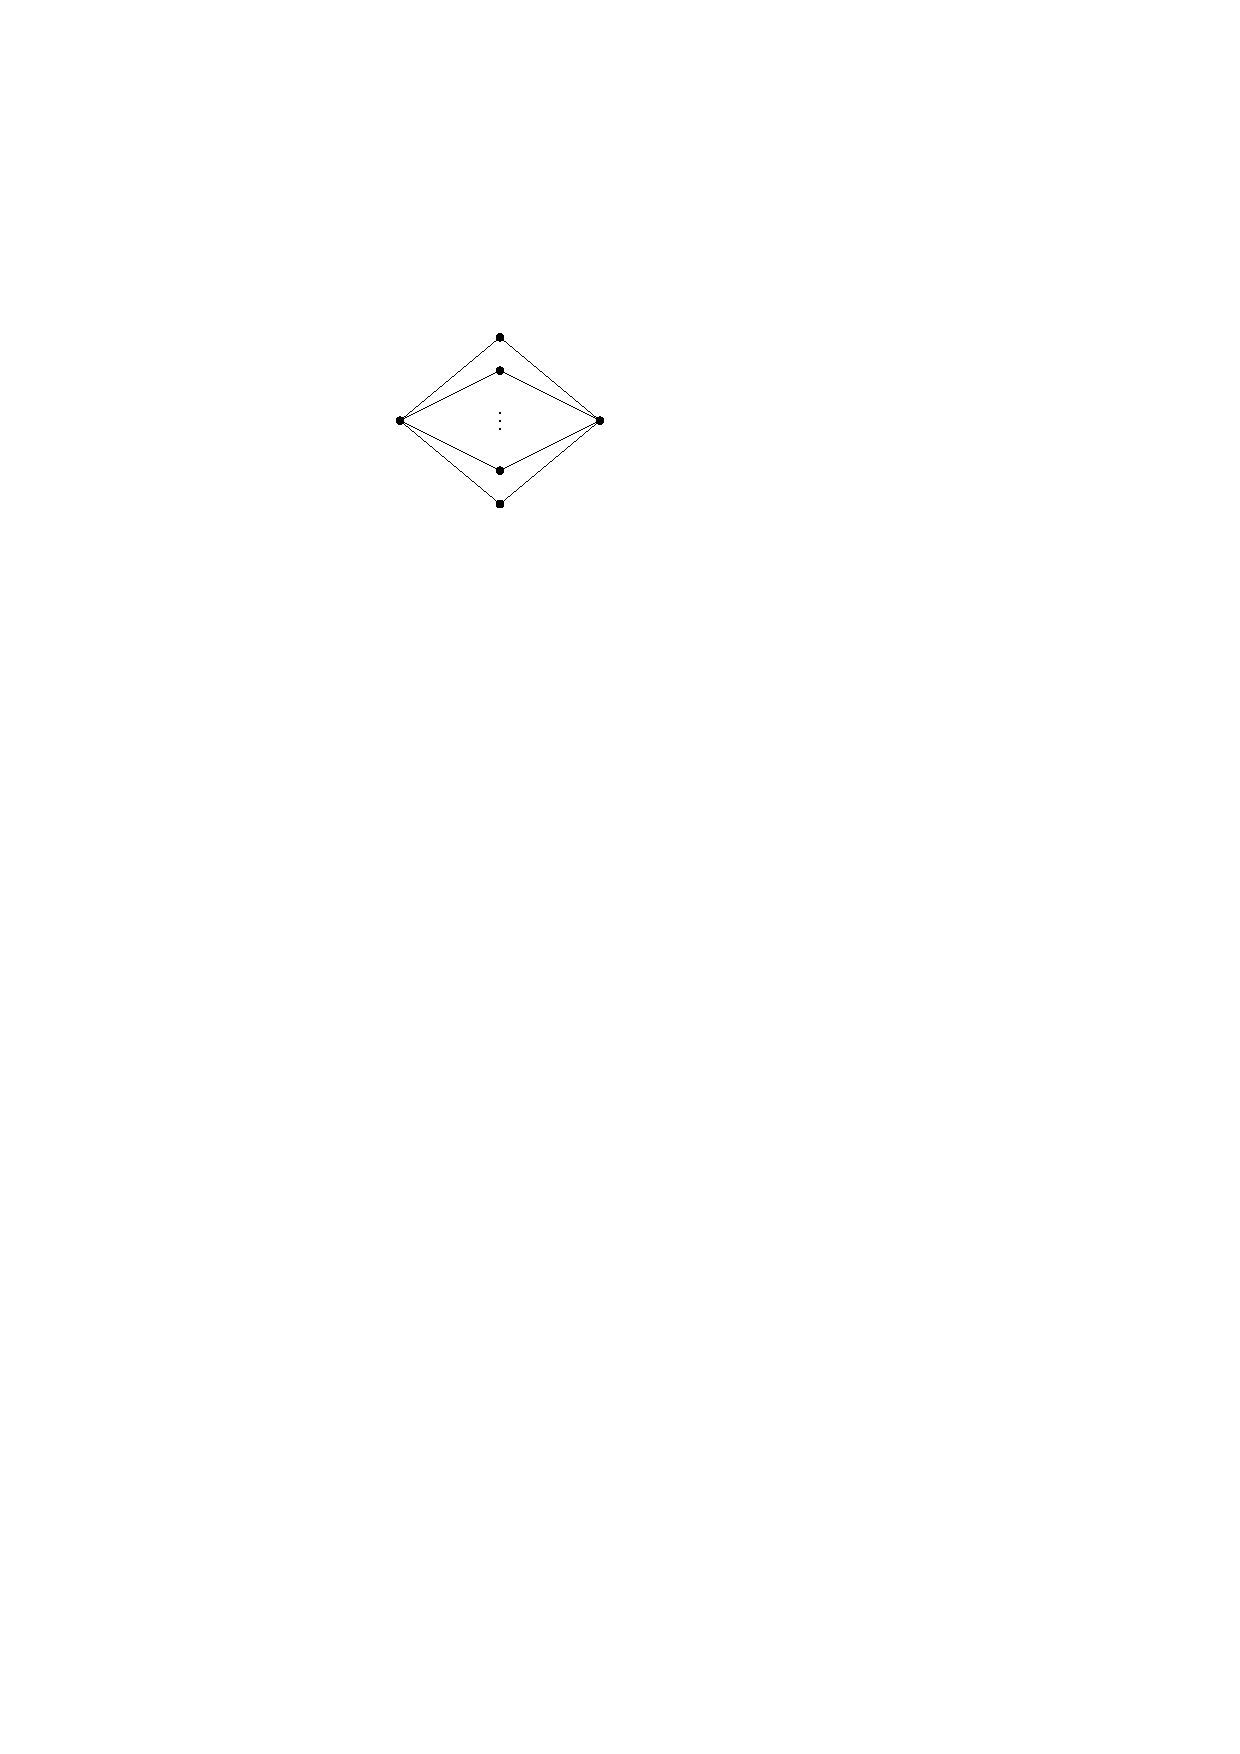
\includegraphics[scale=1]{img/K_2_l}
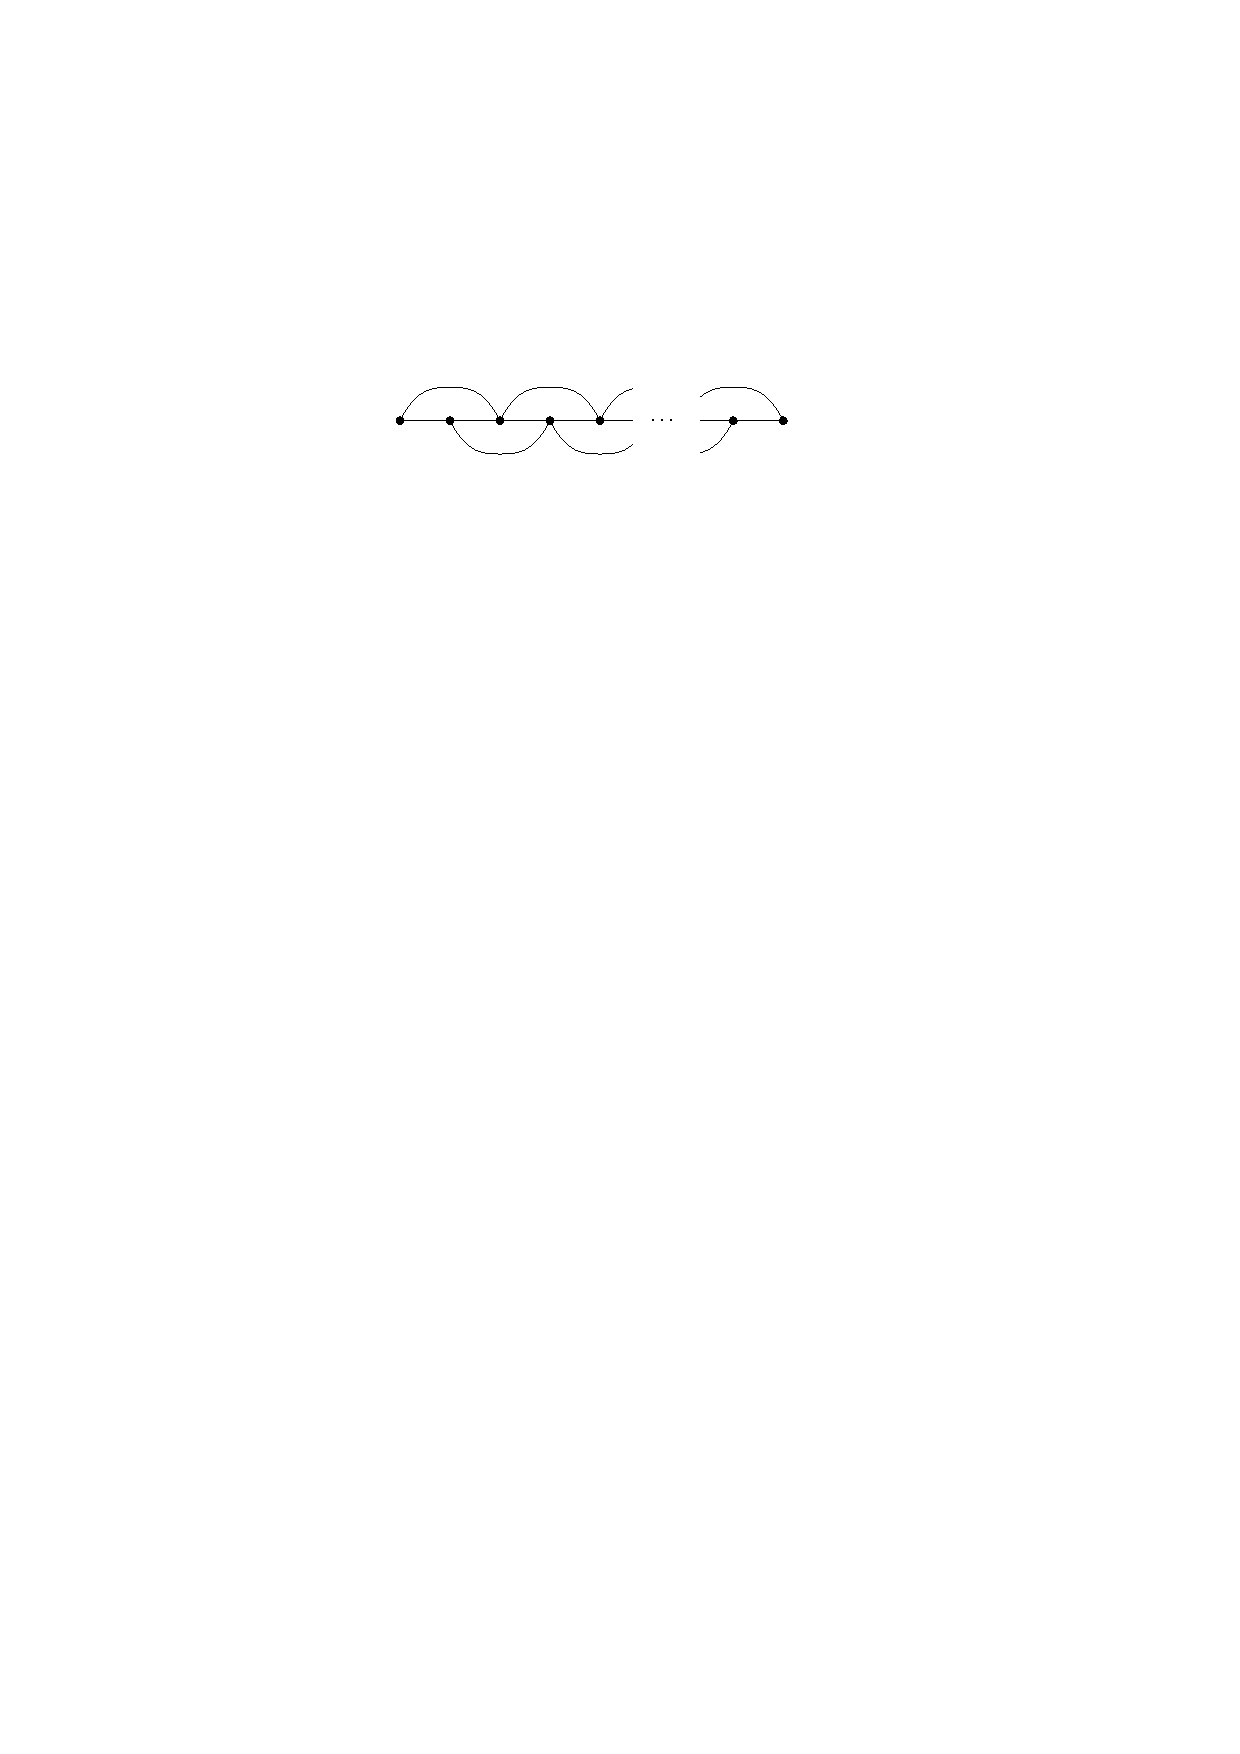
\includegraphics[scale=1]{img/bandwidth_2}
\caption{\lasse{A complete bipartite graph $K_{2,\ell}$ and a graph of bandwidth 2. Problem {\xxxNTP} is NP-hard even on these simple graphs.} }
\label{fig_easy_graphs}
\end{figure}

%%%%%%%%%%%%%%%%%
\begin{theorem}
\label{thm:hardness_complete_bipartite}
Problem {\xxxNTP} is strongly NP-hard, even on complete bipartite graphs $K_{2,\ell}$. 
\end{theorem}
%%%%%%%%%%%%%%%%%
\begin{proof}
Let $q_1,\ldots,q_{3n}$ be an instance of \textsc{3-Partition} as defined above. 
Let $\beta= nQ + n - 1$. 
We construct an instance of {\xxxNTP} on the complete bipartite graph $K_{2,4n-1}$ with bipartition
$\set{a,b}$ and $\set{x_1, \ldots, x_{n-1}, y_1, \ldots, y_{3n}}$. 
For $i\in\{1,\ldots,n-1\}$, we set $w(\set{x_i,a})= i(Q + 1)$ and $w(\set{x_i,b})= (n-i)(Q+1)$. 
For $i\in\{1,\ldots,3n\}$,  we set $w(\set{y_i,a})= q_i$      and $w(\set{y_i,b})= \beta$. 
We claim that the constructed instance of {\xxxNTP} possesses a schedule with objective value $\beta$, 
if and only if the underlying \textsc{3-Partition} instance has answer YES.

(Only if) Assume that for the constructed {\xxxNTP} instance there exists a schedule $\sigma$ 
with objective value $\beta$. 
Note that for every $i \in \{1,\dots,n-1\}$, we have $w(\set{x_i,a}) +w(\set{x_i,b}) = \beta+1$. 
Hence the sum of all the edge weights in the graph is $(n-1)(\beta+1) +3n\beta +(\beta-n+1) = 4\beta n$. 
As every spanning tree for $K_{2, 4n-1}$ has $4n$ edges, each of the connected graphs $G_1,\dots,G_\beta$ 
must have exactly $4n$ edges (and must actually be a spanning tree). \lasse{The fact that the sum of all edge weights is $4\beta n$ furthermore} implies that the activity interval of every edge is contained in $[0, \beta]$.
Now consider some vertex $x_i$ with $i\in\{1,\dots,n-1\}$. 
Since $w(\set{x_i,a}) + w(\set{x_i,b})=\beta+1$, there is exactly one $k\in\fromto{1}{\beta}$ so 
that the edge set $E_k$ contains both edges incident to vertex $x_i$. 
\lasse{Because there are only two possibilities for the two activity intervals of length $w(\set{x_i,a}) = i(Q+1)$ and $w(\set{x_i,b}) = (n-i)(Q+1)$ to cover the whole interval $[0, \beta]$, we see} that either $k=i(Q+1)$ or $k=(n-i)(Q+1)$ holds, and we say that this value $k$ 
is associated with vertex $x_i$.
If some value $k$ is associated with two distinct vertices $x_i$ and $x_j$, then $G_k$ contains 
a cycle; a contradiction.
We conclude that each of the values $k\in\set{Q+1,2(Q+1),\ldots,(n-1)(Q+1)}$ is associated with
exactly one of the vertices $x_1,\ldots,x_{n-1}$.
This means that for the corresponding time slots $[k-1,k]$, vertex $a$ is connected to vertex $b$
via the two edges that are incident to the associated vertex $x_i$.
The remaining $\beta-n+1$ time slots form $n$ (maximal) intervals each of length $Q$.
It is easily verified that during each such interval exactly three vertices $y_i$, $y_j$, $y_{\ell}$
ensure the connection between $a$ and $b$, and that the weights of the three edges $\{y_i,a\}$,
$\{y_j,a\}$, $\{y_{\ell},a\}$ satisfy $q_i+q_j+q_{\ell}=Q$.
Hence the corresponding triplets form a solution for the \textsc{3-Partition} instance.

(If) Now assume that the \textsc{3-Partition} instance has a solution. 
For $1\le i\le n-1$, we activate edge $\set{x_i,a}$ at time~$0$ and edge $\set{x_i,b}$ at time $i(Q+1)-1$.
For $1\le i\le n$, we activate edge $\set{y_i,b}$ at time $0$; finally, the edges $\set{y_i,a}$ are
grouped into triplets according to the solution of the \textsc{3-Partition} instance and scheduled
as indicated in the proof of the (only if) part.
\qed
\end{proof}

%%%%%%%%%%%%%%%%%
\begin{theorem}
\label{thm:hardness_bandwidth}
Problem {\xxxNTP} is strongly NP-hard, even on graphs of bandwidth~$2$.
\end{theorem}
%%%%%%%%%%%%%%%%%
\begin{proof}
Let $q_1,\ldots,q_{3n}$ be an instance of \textsc{3-Partition} as defined above.
We construct an instance of {\xxxNTP} as follows.
The graph $G$ has $4n+1$ vertices $u_0,\ldots,u_n$ and $v_1,\ldots,v_{3n}$.
We will sometimes denote vertex $u_k$ also by the name $v_{k-n}$, for $1\le k\le n+1$;
in particular we use $u_n=v_0$ and $u_{n-1}=v_{-1}$.
Furthermore we define $\beta=(2n-1)Q$.
\begin{itemize}
\item 
For $k=0,\ldots,n-1$,   the edge $\{u_k, u_{k+1}\}$ receives weight $w(\{u_k, u_{k+1}\}) = 2(n-k-1)Q$.
\item
For $k=0,\ldots,n-2$,   the edge $\{u_k, u_{k+2}\}$ receives weight $w(\{u_k, u_{k+2}\})=2(k+1)Q$.
\item 
For $k=1,\ldots,3n$,    the edge $\{v_{k-1}, v_k\}$ has weight $w(\{v_{k-1}, v_k\})=q_k$.
\item
For $k=-1,\ldots,3n-2$, the edge $\{v_k, v_{k+2}\}$ has weight $w(\{v_k, v_{k+2}\})=\beta$.  
\end{itemize}
In the ordering $u_0,u_1,\ldots,u_n,v_1,v_2,\ldots,v_{3n}$, every edge either connects two adjacent 
vertices or two vertices at distance~$2$. Hence, the constructed graph $G=(V,E)$ has bandwidth~$2$. 

We will study schedules $\sigma$ of objective value $\beta$. 
As the sum of all edge weights in $G$ equals $\beta(|V|-1)$, each of the graphs 
$G^\sigma_1, \dots G^\sigma_\beta$ is a spanning tree and the activity interval of every edge is contained in $[0, \beta]$.
We will discuss the behavior of $\sigma$ on the induced subgraph $H_i = G[\fromto{u_0}{u_i}]$ for $1\le i\le n$.
Since the only connections between $H_i$ and the rest of the graph are via the two vertices $u_{i-1}$ and $u_i$,
during any time slot $[t-1,t]$ with $1\le t\le\beta$, graph $H_i$ will consist of one or two connected components
under schedule $\sigma$.
If there is a single connected component, we say that $H_i$ is \emph{fully-connected} during the $t$-th time slot.
If there are two connected components (one containing vertex $u_{i-1}$, the other one containing 
vertex $u_i$), we say that $H_i$ is \emph{semi-connected} during the $t$-th time slot.
Note that if $H_i$ is semi-connected during the $t$-th time slot, then the edge $\{u_{i-1}, u_{i+1}\}$ must be 
active during that slot, as there are no other edges that would be able to connect the component containing 
$u_{i-1}$ to the rest of the graph.

The graph $H_1$ consists of the vertices $u_0$ and $u_1$ and of the edge $\{u_0, u_1\}$ of weight $(2n-2)Q$.
Suppose for the sake of contradiction that $H_1$ is neither fully-connected during the first time slot
nor during the $\beta$-th time slot.
Then the edge $\{u_0, u_2\}$ (of value $2Q$) must be contained both in $E_1$ and in $E_{\beta}$, which is impossible.
By symmetry, we will henceforth assume that under schedule $\sigma$ the graph $G_1$ is fully-connected 
during the $\beta$-th time slot.
This implies that $\{u_0, u_1\}$ is active during $[Q,\beta]$ and that $\{u_0, u_2\}$ is active during $[0,2Q]$.
For graph $H_i$ (with $1\le i\le n$) one can show by induction that $H_i$ is semi-connected
during the time intervals $[0,Q]$, $[2Q,3Q]$, \dots, $[(2i-2)Q,(2i-1)Q]$ and fully-connected at all
other moments in $[0,\beta]$.
The induction uses the following facts and observations on the two edges $\set{u_{i-2}, u_i}$ 
and $\set{u_{i-1},u_i}$ that are in $H_i$ but not in $H_{i-1}$:
\begin{itemize}
\item Graph $H_i$ is semi-connected during the first time slot:
By the inductive hypothesis we have $H_{i-1}$ semi-connected during the first time slot.
If $H_i$ would be fully-connected during the first time slot, we would get
$\sigma(\{u_{i-2}, u_i\}) = \sigma(\{u_{i-1}, u_i\})=0$. 
Since all involved edges have weight $w(e)>Q$, this yields a cycle at time $t=Q+1$ as the desired contradiction.
\item Since graph $H_{i-1}$ is semi-connected at time $0$, the edge $\{u_{i-2},u_i\}$ must be active at 
time $0$ and hence must be active during $[0,(2i-2)Q]$.
\item Graph $H_i$ is fully-connected during the $\beta$-th time slot:
Otherwise, $H_i$ is fully-connected neither during the first time slot nor during the $\beta$-th time slot. 
Then the edge $\{u_{i-1},u_{i+1}\}$ would have to be active for $\beta$ time units.
\item Since $H_i$ is fully-connected during the $\beta$-th time slot, the edge $\{u_{i-1},u_i\}$ must be 
active during the $\beta$-th time slot, and hence must be active during the interval $[(2i-1)Q,\beta]$.
\end{itemize}
The induction yields for $i=n$ that the induced subgraph $H_n$ is semi-connected during the time intervals 
$[0,Q]$, $[2Q,3Q]$, \dots, $[(2n-2)Q,(2n-1)Q]$ (that is, all the intervals of length $Q$ that start at an 
even multiple of $Q$)
and fully-connected during the time intervals $[Q,2Q]$, $[3Q,4Q]$, \dots, $[(2n-3)Q,(2n-2)Q]$ (that is, all the 
intervals of length $Q$ that start at an odd multiple of $Q$).

Next, consider the subgraph $G'$ that is induced by the $3n+2$ vertices $v_{-1}=u_{n-1}$, $v_0=u_n$ and 
$v_1,\ldots,v_{3n}$.
As the edges $\{v_k, v_{k+2}\}$ with $k=-1,\ldots,3n-2$ all have value $\beta$, there is an active path $P_0$ 
through the vertices with even index during the full interval $[0,\beta]$ and there is an active 
path $P_1$ through the vertices with odd index during $[0, \beta]$.
By the above discussion, graph $H_n$ connects these two paths $P_0$ and $P_1$ to each other during the
time intervals $[Q,2Q]$, $[3Q,Q4]$, \dots, $[(2n-3)Q,(2n-2)Q]$.
The only way for connecting $P_0$ and $P_1$ to each other during the remaining time intervals 
$[0,Q]$, $[2Q,3Q]$, \dots, $[(2n-2)Q,(2n-1)Q]$ is by using the edges $\{v_{k-1},v_k\}$ with $k=1,\ldots,3n$ of 
weight $q_k$.
As this groups the numbers $q_1,\ldots,q_{3n}$ into $n$ groups with sum $Q$, we get a solution
for the instance of \textsc{3-Partition}.

Vice versa, if the \textsc{3-Partition} instance has a solution, then we  build a schedule $\sigma$
of objective value $\beta$: For $k=0,\ldots,n-1$, we activate edge $\set{u_k, u_{k+1}}$ at time $(2k+1)Q$. For $k=0,\ldots,n-2$, we activate edge $\set{u_k, u_{k+2}}$ at time $0$. For $k=-1,\ldots,3n-2$, we activate edge $\set{v_k, v_{k+2}}$ at time $0$. Finally, the edges $\set{v_{k-1},v_k}$ are grouped into triplets and scheduled as described in the other direction of the proof.
\qed
\end{proof}


%%%%%%%%%%%%%%%%%%%%%%%%%%%%%%%%%%%%%%%%%%%%%%%%%%%%%%%%%%%%%%%%%%%%%%%%%
%%%%%%%%%%%%%%%%%%%%%%%%%%%%%%%%%%%%%%%%%%%%%%%%%%%%%%%%%%%%%%%%%%%%%%%%%
\section{A Negative Result for Objective Value Seven}
\label{sec:value-seven}
%%%%%%%%%%%%%%%%%%%%%%%%%%%%%%%%%%%%%%%%%%%%%%%%%%%%%%%%%%%%%%%%%%%%%%%%%
In this section, we show that it is NP-hard to decide whether there exists a schedule of objective value at least 7. 
The reduction is from the following version of the Hamilton cycle problem; 
see Akiyama, Nishizeki \& Saito \cite{hamilton3regularBip}
%%%%%%%%%%%%%%%%%%%%%%%%%%
\begin{quote}
Problem {\xxxHAM}
\\
\textbf{Instance:} A bipartite, 3-regular graph $H'$.  
\\
\textbf{Question:} Does $H'$ possess a Hamilton cycle? 
\end{quote}
%%%%%%%%%%%%%%%%%%%%%%%%%%
The reduction is done in two steps.
The first step transforms an instance $H'$ of {\xxxHAM} into a new 4-regular graph $H$ 
with the properties described in Lemma~\ref{le:Ham-to-Ham}.
\lasse{(Roughly speaking, we transform $H'$ into a graph $H$ where the existence of a Hamilton path and a Hamilton cycle are equivalent, because we require a Hamilton cycle for one direction of the reduction, but can only show the existence of a Hamilton path in the other direction.)}
The second step then transforms the 4-regular graph $H$ from Lemma~\ref{le:Ham-to-Ham}
into a corresponding instance of problem {\xxxNTP}.

%%%%%%%%%%%%%%%%%
\begin{lemma}
\label{le:Ham-to-Ham}
There is a polynomial time algorithm that takes an instance $H'$ of {\xxxHAM} as input and outputs 
a 4-regular bipartite graph $H$ together with an edge $\{u,z\}\in E(H)$ \lasse{(which we call the \emph{special edge})},
so that the following holds:
\begin{enumerate}[(i)]
\item If $H'$ is a YES-instance of {\xxxHAM}, then the new graph $H$ contains a Hamilton cycle 
that traverses the special edge $\{u,z\}$.
\item If $H'$ is a NO-instance of {\xxxHAM}, then the new graph $H$ has no Hamilton path
starting in vertex $u$. 
\end{enumerate}
\end{lemma}

\begin{proof}
\lasse{
The reduction is sketched in \cref{fig_hamilton_cycle_lemma}. Let $H' = (V, E)$. The algorithm chooses some arbitrary vertex $x \in V$. The graph $H$ then consists out of the following components: There are two copies of $H'$, called $H'_1$ and $H'_2$ respectively. For each vertex $v \in V$, we denote by $v_1$ its copy in $H'_1$ and by $v_2$ its copy in $H'_2$. For each vertex $v \in V-\set{x}$, we take a copy $A_v$ of $K_{4,4}$, remove some edge $\set{u_1, u_2}$ from $A_v$, and add edges $\set{v_1,u_1}$ and $\set{u_2,v_2}$. Finally, we take two copies $A_x$ and $A'_x$ of $K_{4,4}$, remove an edge $\set{u_1,u_2}$ from $A_x$ and an edge $\set{u'_1,u'_2}$ from $A'_x$, add edges $\set{x_1,u_1}$, $\set{u_2,u'_1}$, $\set{u'_2,x_2}$. The special edge is given by $\set{u, z}$ with $u := u_2$, and $z := u'_1$. Clearly, $H$ is bipartite and 4-regular, so it remains to prove claims (i) and (ii).
}
\begin{figure}[htpb]
\centering
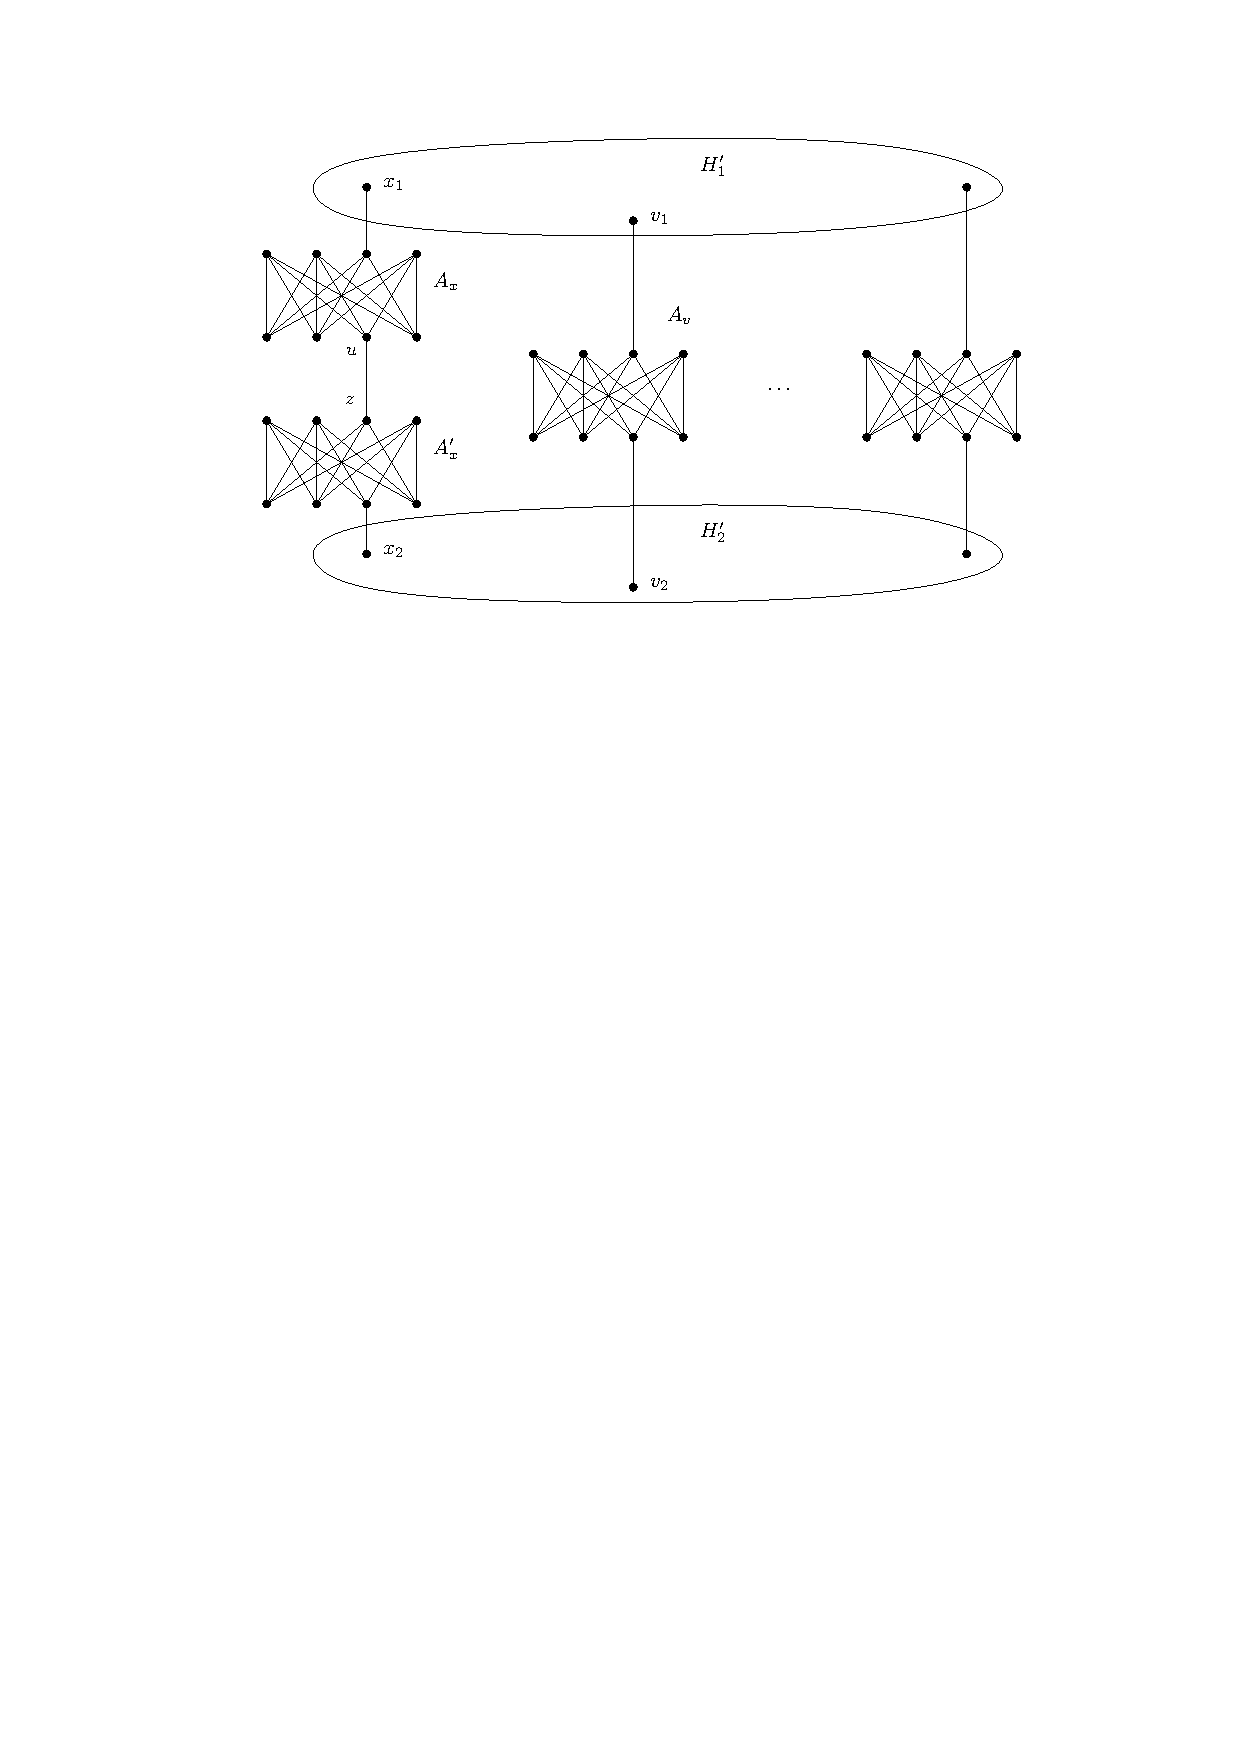
\includegraphics[scale=0.92]{img/hamilton-prime}
\caption{\lasse{Construction used in the proof of \cref{le:Ham-to-Ham}.}}
\label{fig_hamilton_cycle_lemma}
\end{figure}

\lasse{
For claim (i), assume that $H'$ has a Hamilton cycle $C'$. Then we obtain a Hamilton cycle $C$ in $H$ using the edge $\set{u,z}$ in the following fashion: We start at the vertex $u$, and traverse all the vertices of $A_x$ in such an order that we can go afterwards to $x_1$. Then we go to $x_1$. Now we follow the edges of the cycle $C'$ alternatingly in $H'_1$ and $H'_2$. Precisely, whenever we follow an edge of $C'$ to encounter a new vertex $v_1$ ($v_2$, respectively), we traverse all the vertices of $A_v$ and go to $v_2$ ($v_1$, respectively) and then follow the next edge of $C'$. Because the graph $H'$ has an even number of vertices (it is bipartite and 3-regular), we will end up at $x_2$. We then complete the tour by traversing all vertices of $A'_x$ and going along the edge $\set{u,z}$ at the end. This describes a Hamilton cycle of $H$ which uses the edge $\set{u,z}$.
}

\lasse{
For claim (ii), we prove the contrapositive. Assume that $H$ has a Hamilton path $P = (w_1,\dots,w_n)$ starting at vertex $u$, we have to prove that $H'$ has a Hamilton cycle. Note that if $w_2 = z$, then $w_n$ is in $A_x$. On the other hand, if $w_2$ is in $A_x$, then $w_n$ is in $A'_x$. We first assume that $w_2 \in A_x$ and $w_n \in A'_x$.
We claim that the Hamilton path $P$ necessarily switches between $H'_1$ and $H'_2$ after every of its edges in $H'_1$ or $H'_2$. Indeed, let $v \neq x$ be a vertex of $H'$ and assume without loss of generality that from the two vertices $v_1$ and $v_2$ the path $P$ first encounters $v_1$. If the path does not immediately switch to $v_2$, then it will at a later stage need to visit $v_2$. But in this case, it has to visit $A_v$ after visiting $v_2$, in contradiction to the fact that the path has to return to $A'_x$. This proves that $P$ switches between $H'_1$ and $H'_2$ after every egde in $H'_1$ or $H'_2$. Then looking at the edges of $P$ which lie in $H'_1$ or $H'_2$, we see that $H'$ has a Hamilton cycle. Finally, an anologous statement holds in the case $w_2 = z$. So we have proven the claim. \qed
}
\end{proof}


%%%%%%%%%%%%%%%%%

\begin{figure}[htpb]
\centering
 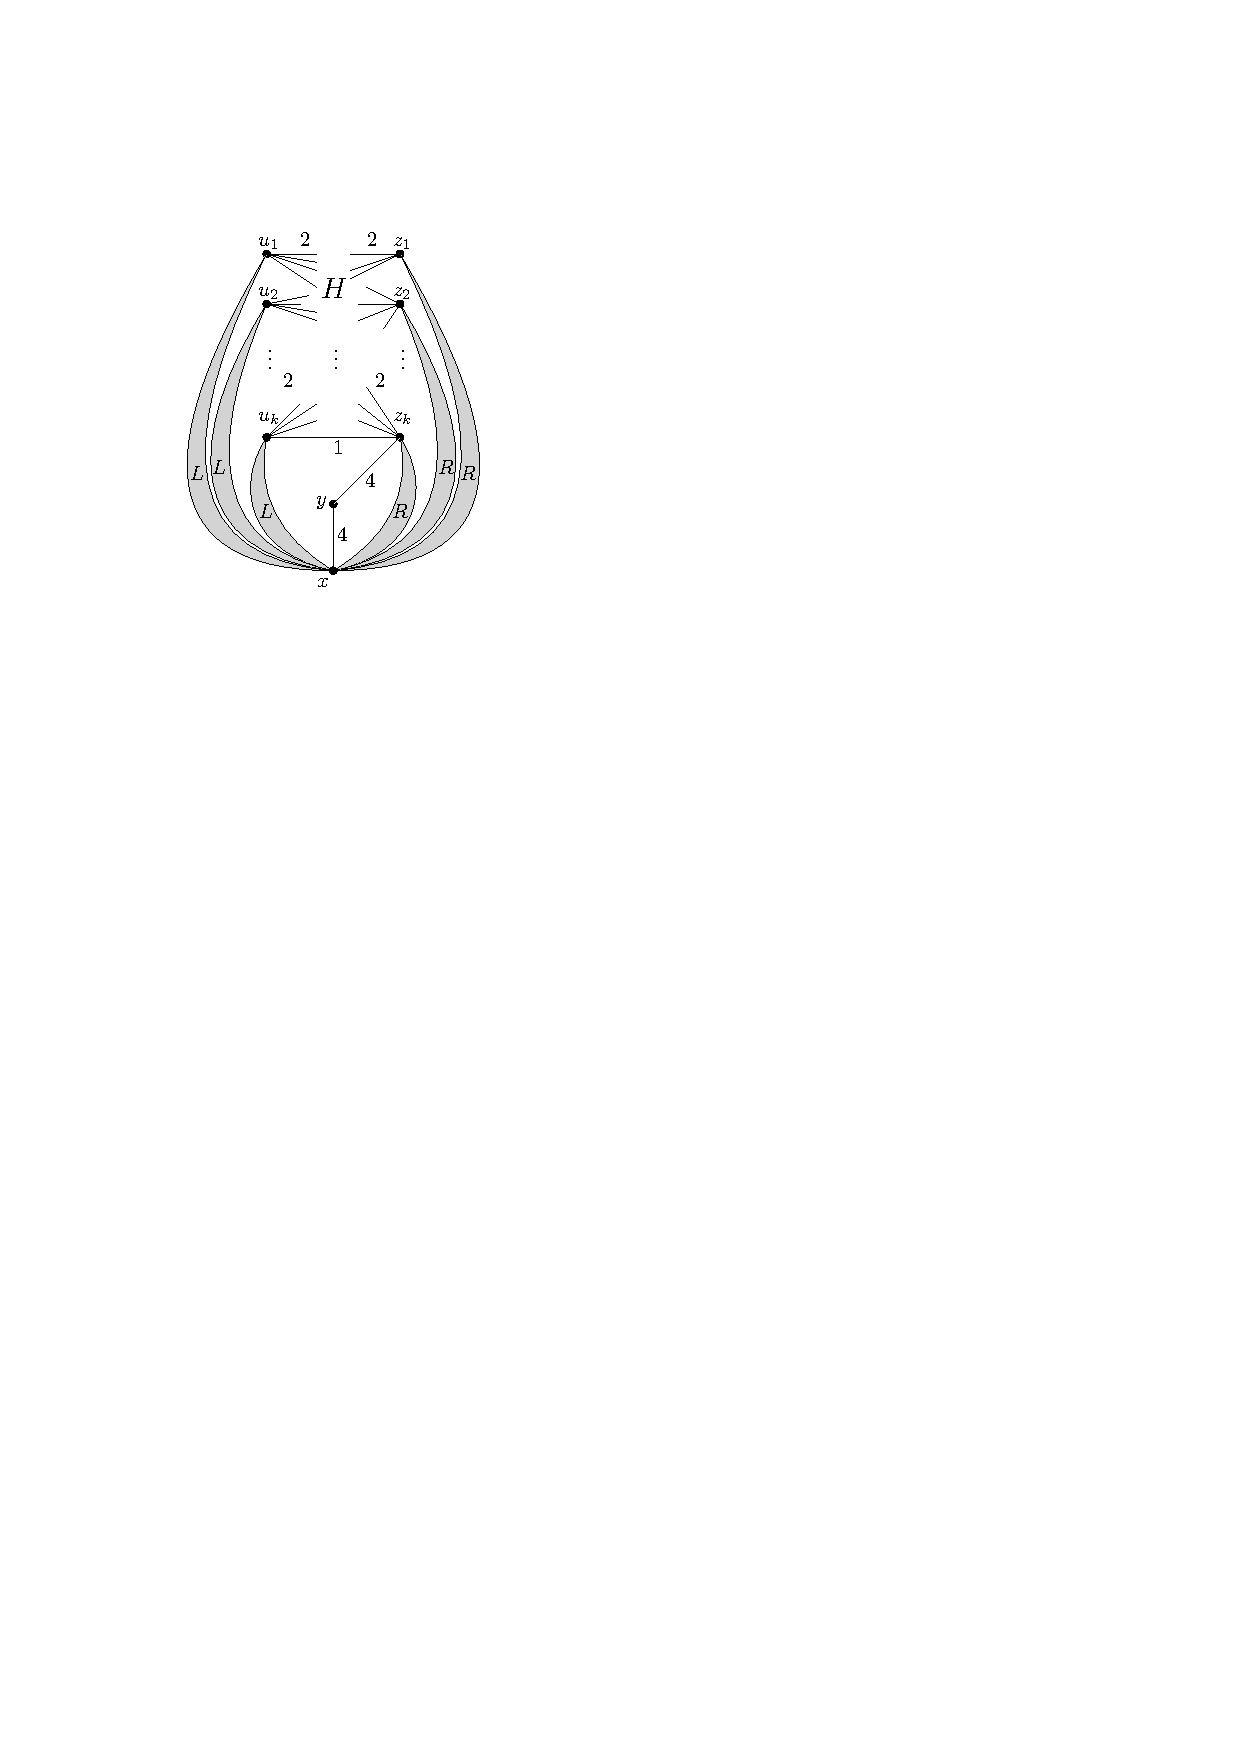
\includegraphics[scale=1.1]{img/act-hamilton-cycle-a}
\caption{Sketch of the {\xxxNTP} instance $(G, w)$ obtained from the 4-regular bipartite graph $H$.}
\label{fig:reduction-overview}
\end{figure}
Now let $H$ be a 4-regular bipartite graph as described in Lemma~\ref{le:Ham-to-Ham}.
Let $U=\fromto{u_1}{u_k}$ and $Z=\fromto{z_1}{z_k}$ denote the two parts in the bipartition of $H$, 
and let $\{u_k,z_k\}$ be its special edge.
We create an instance $(G,w)$ of {\xxxNTP} from $H$. An informal sketch of this instance $(G,w)$ is depicted in \cref{fig:reduction-overview}. Formally, it is described the following way:
The graph $G$ has the vertex set 
%%%%%%%%%%%%%%%%%
\[ 
V(G) =  \set{x, y} \cup U \cup Z 
        \cup \bigcup_{i=1}^k \fromto{v_{i1}}{v_{i4}} \cup \bigcup_{i=1}^k \set{v'_{i1}, v'_{i2}}.
\]
%%%%%%%%%%%%%%%%%
Furthermore, the graph $G$ has the following edges and edge weights:
\begin{itemize}
\item \lasse{Between the vertex sets $U$ and $Z$, the graph $G$ has exactly the same edges as the graph $H$. 
For every such edge $e$, we set} $w(e) = 2$, if $e \neq \set{u_k, z_k}$ and $w(\set{u_k, z_k}) = 1$.
\item For every $i = 1,\dots,k$, the induced subgraph $L_i = G[\set{x, u_i, v_{i1}, v_{i2}, v_{i3}, v_{i4}}]$ 
is called the \emph{$i$-th gadget of type L} and has edges and edge weights as depicted in \cref{fig:act-hamilton-cycle}.
\item For every $i = 1,\dots,k$, the induced subgraph $R_i = G[\set{x, z_i, v'_{i1}, v'_{i2}}]$ is called the 
\emph{$i$-th gadget of type R} and has edges and edge weights as depicted in \cref{fig:act-hamilton-cycle}.
\item Finally, the two edges $\set{x,y}$ and $\set{y, z_k}$ have $w(\set{x,y}) = w(\set{y, z_k}) = 4$. The induced subgraph $G[\set{x,y,z_k}]$ is called the \emph{gadget $C$}.
\end{itemize}
%%%%%%%%%%%%%%%%%%%%%%%%%%
\begin{figure}[htpb]
\centering
 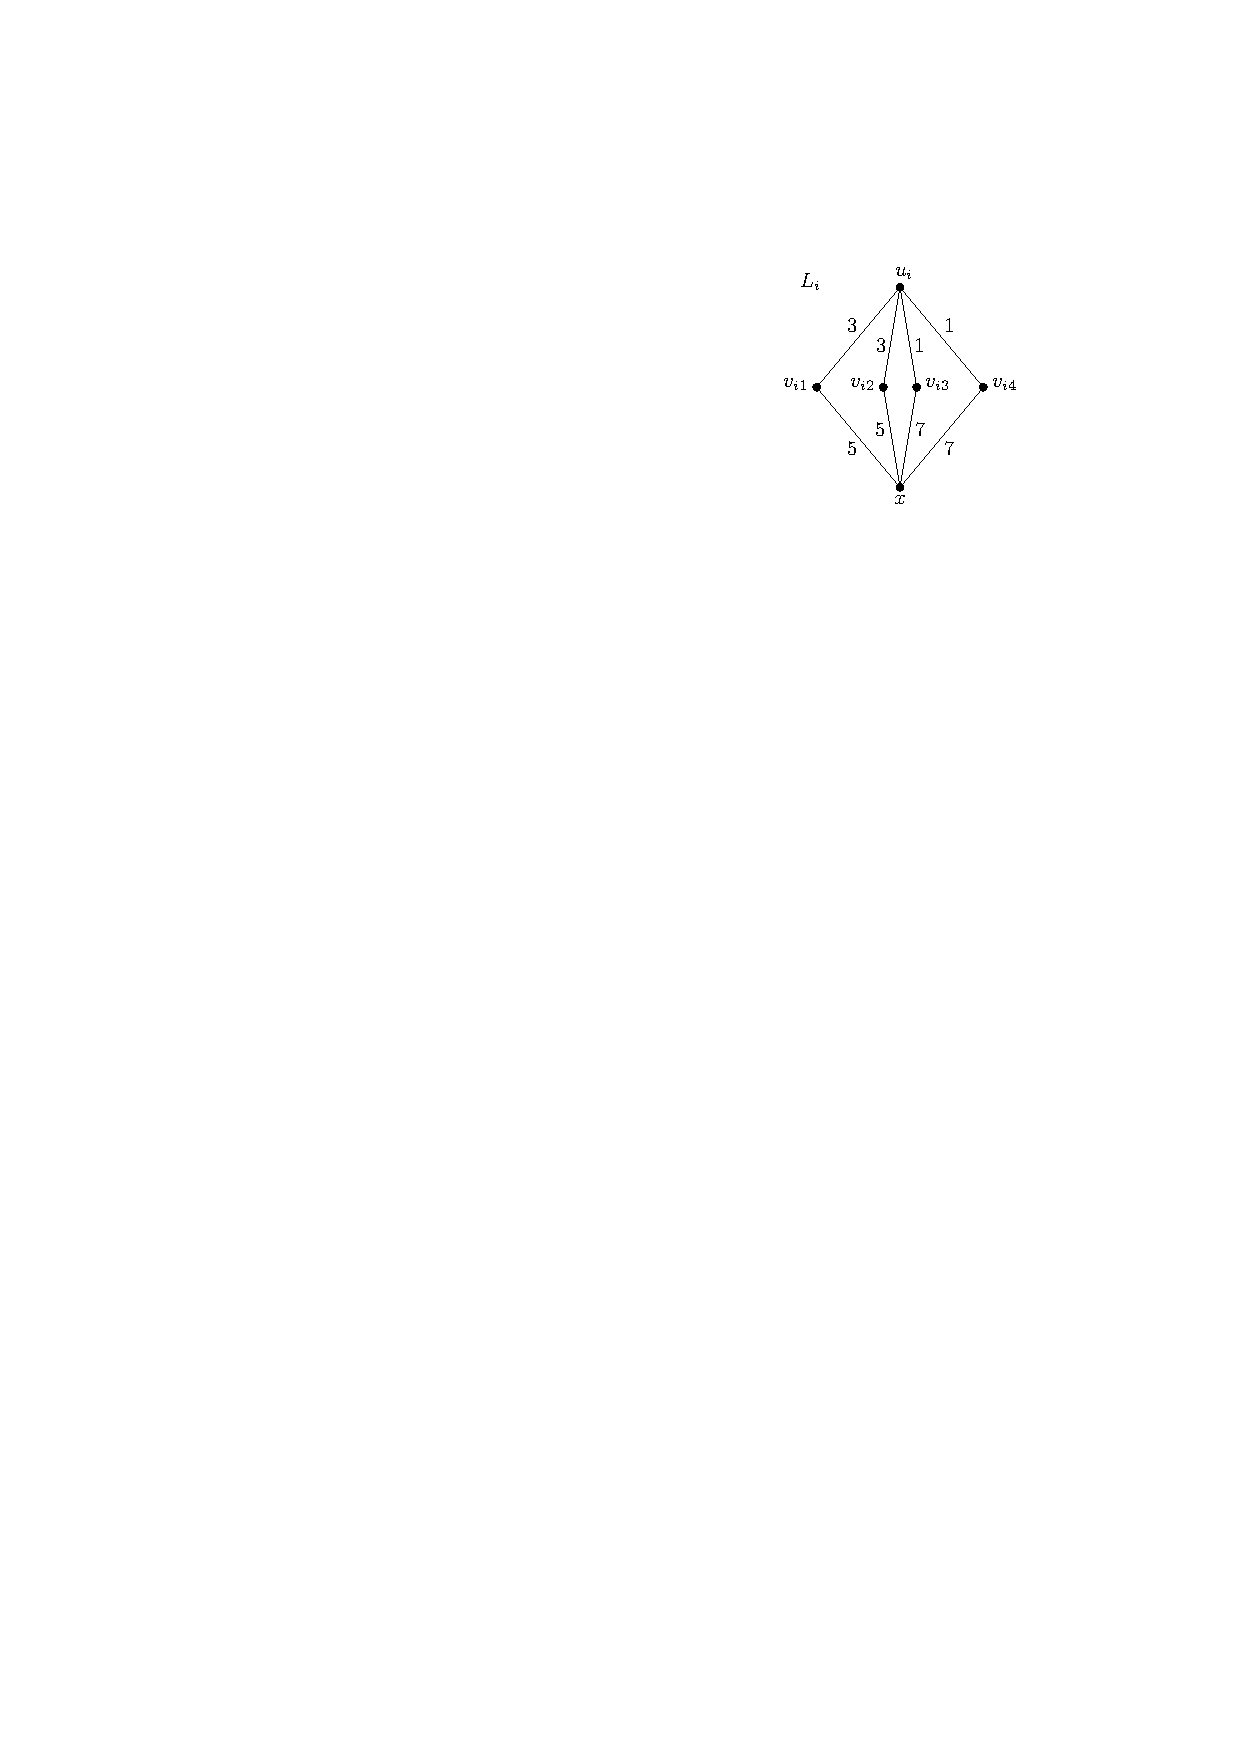
\includegraphics[scale=1.1]{img/act-hamilton-cycle-b-simplified}
\qquad\qquad\qquad
 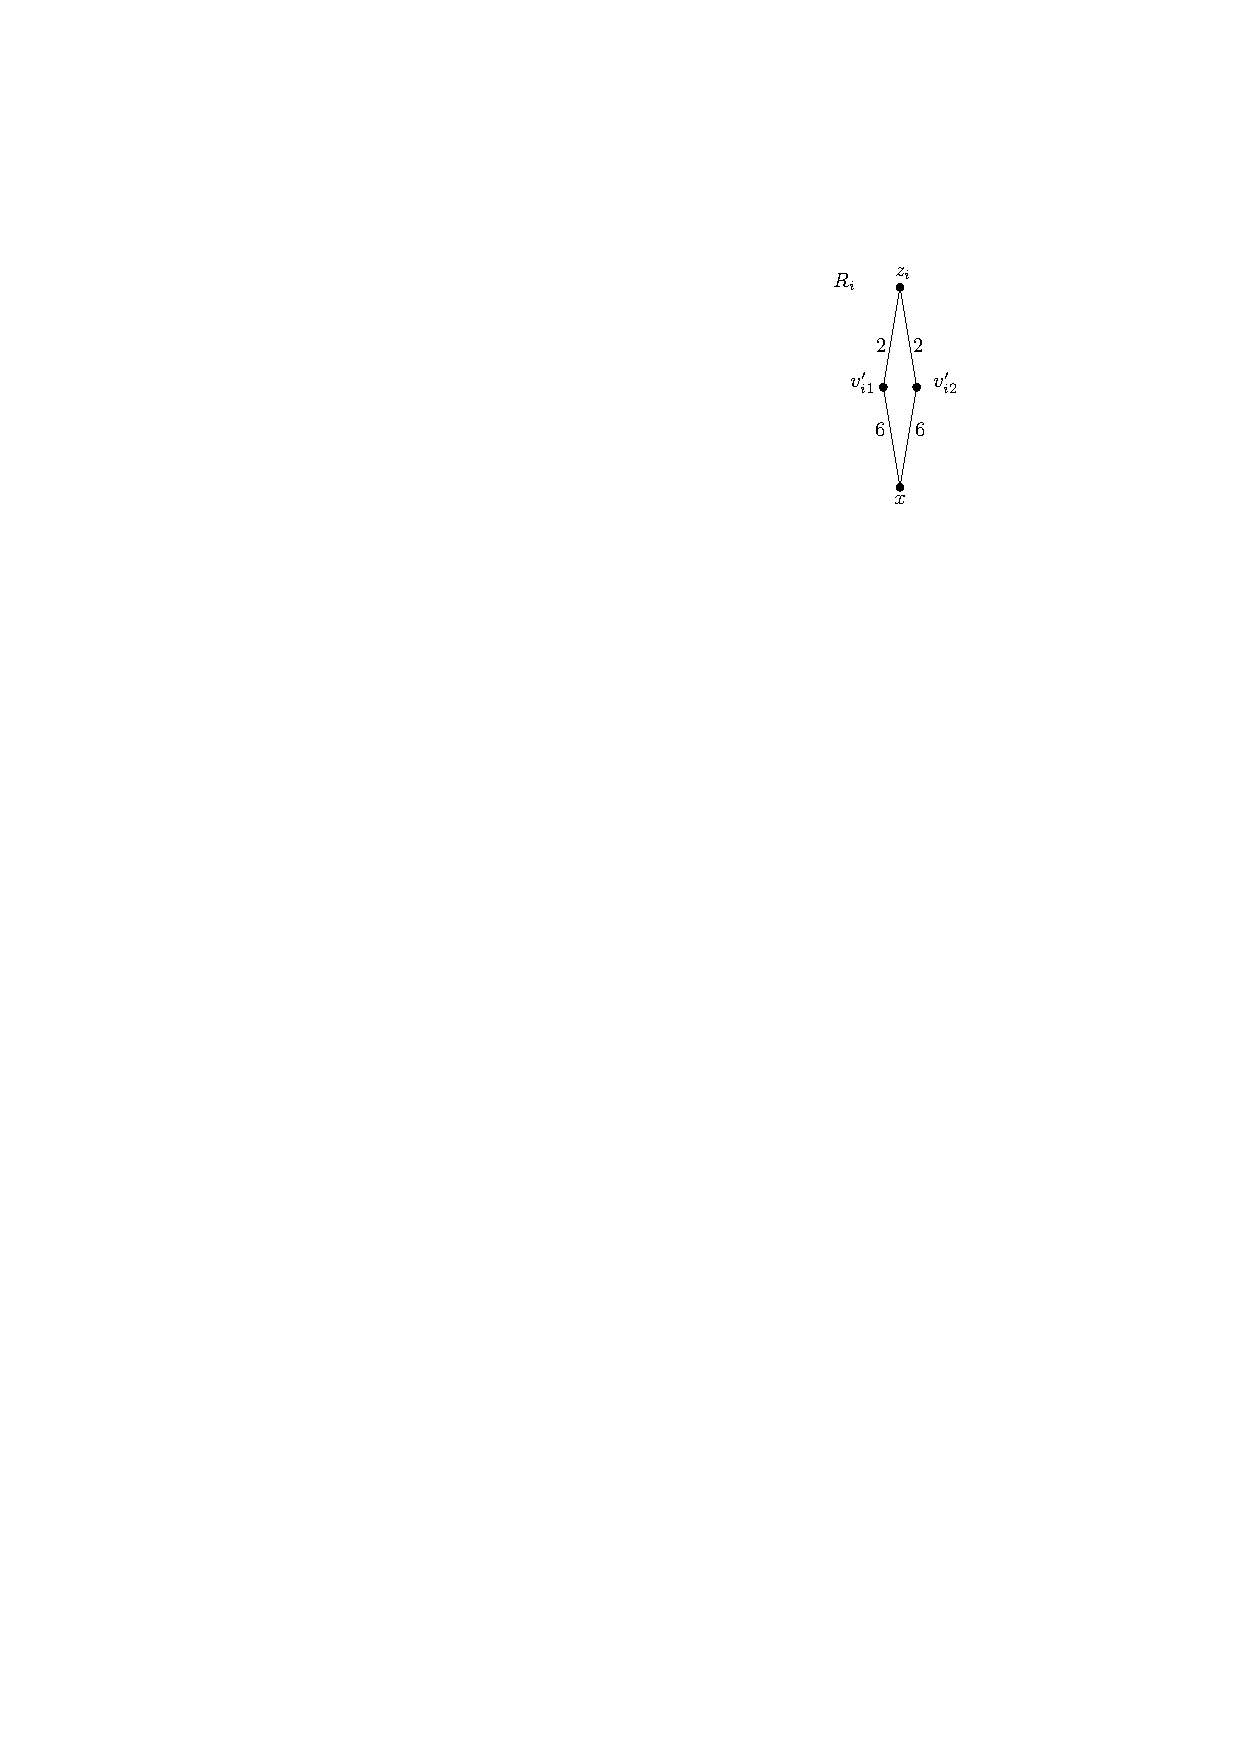
\includegraphics[scale=1.1]{img/act-hamilton-cycle-c}
\caption{Gadget of type $L$ (on the left) and gadget of type $R$ (on the right).}
\label{fig:act-hamilton-cycle}
\end{figure}
%%%%%%%%%%%%%%%%%%%%%%%%%%
Now assume that $(G, w)$ allows some schedule $\sigma$ of objective value 7. 
During any time slot $[t-1,t]$ with $1\le t\le7$, the $i$-th gadget of type $L$ will 
consist of either one or two connected components under schedule $\sigma$. 
If there is a single connected component, we say that $L_i$ is \emph{fully-connected} during the $t$-th time slot. If there are two connected components (one containing  $x$, and one containing $u_i$), we say that $L_i$ is \emph{semi-connected} during the $t$-th time slot. In the same manner, during the $t$-th time slot, gadget $R_i$ is either fully-connected or semi-connected with $x$ and $z_i$ in different components. Likewise, the gadget $C$ is either fully-connected, or semi-connected with $x$ and $z_k$ in different components.

\begin{lemma}
\label{lemma:gadgets_properties}
Let $(G,w)$ be the instance described above. 
Every schedule of objective value 7 for $(G, w)$ satisfies the following.
\begin{enumerate}[(i)]
\item A gadget of type $R$ is fully-connected during time slots 2 and 6, and 
semi-connected during each of the remaining five time slots.
\item For each $i=1,\dots,k$, there are $t_1,t_2 \in \set{1,2,4,6,7}$ with $t_1\ne t_2$, such that the gadget $L_i$ is fully-connected during time slots $3,5,t_1, t_2$, 
and semi-connected during each of the remaining three time slots.
\item The gadget $C$ is fully-connected during time slot 4, 
and semi-connected during each of the remaining six time slots.
\end{enumerate}
\end{lemma}
\begin{proof}
Note that the sum of all edge weights in $G$ is $8k-1 +32k +16k +8 = 56k+7 = 7(8k + 1) = 7(|V(G)|-1)$. 
This implies that each of the graphs $G_1,\ldots,G_7$ is a tree (in particular, it is acyclic) and that the activity interval of each edge is contained in $[0, \beta]$.
For the proof of (i), consider the vertex $v'_{i1}$ in the gadget $R_i$. 
There is exactly one time slot $[t-1, t]$ during which both edges incident to $v'_{i1}$ are active, 
and we have $t=2$ or $t=6$. 
Analogously, there is exactly one time slot $[t'-1, t']$ during which both edges incident to 
the vertex $v'_{i2}$ are active, and we have $t' = 2$ or $t' = 6$. 
As $t=t'$ yields the contradiction that $G_t$ has a cycle, we conclude $\set{t,t'}=\set{2,6}$ and (i) follows. 
Claims (ii) and (iii) can be proven in the same manner. 
\qed
\end{proof}

\begin{lemma}
\label{lemma:lasse-if}
Let the graph $H$ and the special edge $\set{u,z}$ be as described in \cref{le:Ham-to-Ham}, and let $(G, w)$ be the corresponding {\xxxNTP} instance. 
If $H$ contains a Hamilton cycle which uses the special edge, then $\ntp(G, w) \geq 7$.
\end{lemma}
\begin{proof}
Let $e_0 = \set{u, z} = \set{u_k, z_k}$ be the special edge. There is a Hamilton cycle $W$ using $e_0$. Then the graph $H-E(W)$ is 2-regular, hence there exist pairwise disjoint matchings $M_1, \ldots, M_4$ such that $M_1 \dotunion M_2 = E(W)$ and $M_3 \dotunion M_4 = E(H) - E(W)$ and $e_0 \in M_1$. We describe a schedule $\sigma$ with objective value 7:
\begin{itemize}
\item All gadgets of type $R$ are fully-connected during time slots 2 and 6, and semi-connected otherwise.
\item All gadgets of type $L$ are fully-connected during time slots 1, 3, 5, and 7, and semi-connected otherwise.
\item The gadget $C$ is fully-connected during time slot 4, and semi-connected otherwise.
\item All edges $e \in M_1 - \set{e_0}$ have activity interval $[2, 4]$. The edge $e_0$ has activity interval $[2, 3]$.
\item All edges $e \in M_2$ have activity interval $[3, 5]$.
\item All edges $e \in M_3$ have activity interval $[0, 2]$.
\item All edges $e \in M_4$ have activity interval $[5, 7]$.
\end{itemize}
It is easy to see that a schedule $\sigma$ with these properties does indeed exist. \cref{table:lasse-if} provides a schematic description of the schedule, by indicating for each number $t$, which edges are scheduled and which gadgets are fully connected during the the $t$-th time slot $[t-1, t]$.  Notice that the active edges in $H$ form a matching of $H$ during the time slots 1,2,3,5,6, and 7, 
and form a Hamilton path of $H$ during the time slot 4. 
By checking each of the cases $t=1,\dots,7$, it is easily seen that each of the graphs $G^\sigma_1,\ldots,G^\sigma_7$ is connected. We therefore conclude that $\ntp(\sigma) = 7$. 
\begin{table}[htpb]
\centering
 \begin{tabular}{ c | c | c | c | c | c | c } 
 \multicolumn{7}{c}{time slot}\\
	1 & 2 & 3 & 4 & 5 & 6 & 7 \\
	\hline
	 & $R$ & & & & $R$ & \\
	 $L$ & & $L$ & & $L$ &  & $L$ \\
	 & & & $C$ & & &  \\
	 & & $M_1$ & $M_1 - \set{e_0}$  & & &  \\
	  & & & $M_2$  & $M_2$ & &  \\
	  $M_3$ & $M_3$ & &  &  & &  \\
	   & & &  &  & $M_4$ & $M_4$ 
 \end{tabular}
 \caption{Description of the schedule $\sigma$ from \cref{lemma:lasse-if}.}
 \label{table:lasse-if}
\end{table}
\qed
\end{proof}

\begin{lemma}
\label{lemma:lasse-only-if}
Let the graph $H$ and the special edge $\set{u,z}$ be as described in \cref{le:Ham-to-Ham}, and let $(G, w)$ be the corresponding {\xxxNTP} instance. If $\ntp(G, w) \geq 7$, then $H$ contains a Hamilton path starting at vertex $u$.
\end{lemma}
\begin{proof}
So assume there exists a schedule $\sigma$ of objective value 7. 
For a vertex $v \in U \cup Z$, and $t \in \fromto{1}{7}$, let $d_t(v) = |\delta(v) \cap E(H) \cap E_t|$ denote the number of incident edges of $v$, which are both in $E(H)$ and active during the $t$-th time slot. The strategy of the proof will be to repeatedly deduce some conditions for $d_t(v)$. 
Let $e_0 = \set{u, z} = \set{u_k, z_k}$ be the special edge.

First, recall \cref{lemma:gadgets_properties}. Consider vertex $z_i$ for some $i \in \fromto{1}{k}$. We know that for each $t \in \set{1, 3, 5, 7}$ in the $t$-th time slot both the gadget $R_i$ and the gadget $C$ are semi-connected. But of course at least one edge incident to $z_i$ must be active during the $t$-th time slot. Hence $d_1(z_i), d_3(z_i), d_5(z_i), d_7(z_i) \geq 1$.  Note that the four edges in $\delta(z_i) \cap E(H)$ each have weight at most 2 (in the case $i \neq k$ we have four times weight 2, and for $i = k$ we have three times weight 2, and $w(e_0) = 1$). For the sake of contradiction, assume $d_1(z_i) > 1$. Then from the four edges in $\delta(z_i) \cap E(H)$ at least two are scheduled at time $0$. This is a contradiction to  $d_3(z_i), d_5(z_i), d_7(z_i) \geq 1$. Hence $d_1(z_i) = 1$. By the same argument, $d_7(z_i) = 1$. A similar argument shows that $e_0 \not\in E_4$.

Next, consider the graph $G_1$ of active edges in the first time slot. We know that  $d_1(z_i) = 1$ for all $i= 1,\dots, k$. Hence the induced subgraph $G_1[U \cup Z]$ on $2k$ vertices is acyclic, has $k$ edges, and therefore has $k$ connected components. But because $G_1$ is connected, and because all the gadgets of type $R$ and the gadget $C$ are semi-connected during time slot 1, this implies that every single gadget of type $L$ is actually fully-connected during time slot 1. The same argument holds for time slot 7. In total, together with \cref{lemma:gadgets_properties}, we have that a gadget of type $L$ is fully-connected during the $t$-th time slot, if and only if $t \in \set{1, 3, 5, 7}$. This in turn implies that for all $i = 1,\dots, k$, one has $d_2(u_i), d_4(u_i), d_6(u_i) \geq 1$. The two facts $d_2(u_i) \geq 1$ and $d_6(u_i) \geq 1$ together imply $d_4(u_i) \leq 2$. Likewise, for all $i = 1,\dots,k$, the two facts $d_1(z_i) = 1$ and $d_7(z_i) = 1$ together imply $d_4(z_i) \leq 2$.

Finally, we claim $d_4(u_k) = 1$. In fact, $d_4(u_k) = 0$ is impossible, because gadgets of type $L$ are semi-connected during time slot 4. For the sake of contradiction, assume $d_4(u_k) > 1$. We know that $d_2(u_k) \geq 1, d_6(u_k) \geq 1$ and $e_0 \not\in E_4$ and $w(e_0) = 1$. So our assumption $d_4(u_k) > 1$ is only possible if $e_0 \in E_2$ or $e_0 \in E_6$. But for the vertex $z_k$, we also know $d_1(z_k), d_3(z_k), d_5(z_k), d_7(z_k) \geq 1$. This is a contradiction to $e_0 \in E_2 \cup E_6$, hence our assumption was wrong and $d_4(u_k) = 1$.
In summary, during time slot 4, all gadgets of type $L$ and $R$ are semi-connected. We also have for all $i=1,\dots,k$ that $d_4(u_i) \leq 2$ and $d_4(z_i) \leq 2$. Also, $d_4(u_k) = 1$. However, $G_4$ is connected. These facts together imply that the induced subgraph $G_4[U \cup Z]$ is a Hamilton path in $H$ starting at $u_k = u$.
\qed
\end{proof}

By combining \cref{le:Ham-to-Ham,lemma:lasse-only-if,lemma:lasse-if} we get
the following summarizing theorem.
%%%%%%%%%%%%%%%%%%%%%%%%%%
\begin{theorem}
\label{th:value=7}
For {\xxxNTP} it is strongly NP-hard to decide whether there exists a schedule
of objective value at least~$7$.
\qed
\end{theorem}
%%%%%%%%%%%%%%%%%%%%%%%%%%

All edge weights in the above reduction are in the set $\fromto{1}{7}$.
A minor modification yields the following corollary.
%%%%%%%%%%%%%%%%%%%%%%%%%%
\begin{restatable}{corollary}{weightsOneToSix}
\label{coro:small-weights}
Problem {\xxxNTP} is strongly NP-hard, even if all edge weights are in $\fromto{1}{6}$.
\end{restatable}
\begin{proof}
Edges of weight~$7$ only show up in the gadget of type $L$.
Figure~\ref{fig_hamilton_cycle_improved} shows a modified version of this gadget that emulates 
the edges of weight~$7$ by edges with weights in $\fromto{1}{6}$.
One easily verifies that the functionality of the gadget remains the same and that in particular
Lemma~\ref{lemma:gadgets_properties} still holds true.
\qed
\end{proof}
%%%%%%%%%%%%%%%%%%%%%%%%%%
%%%%%%%%%%%%%%%%%%%%%%%%%%
\begin{figure}[htpb]
\centering
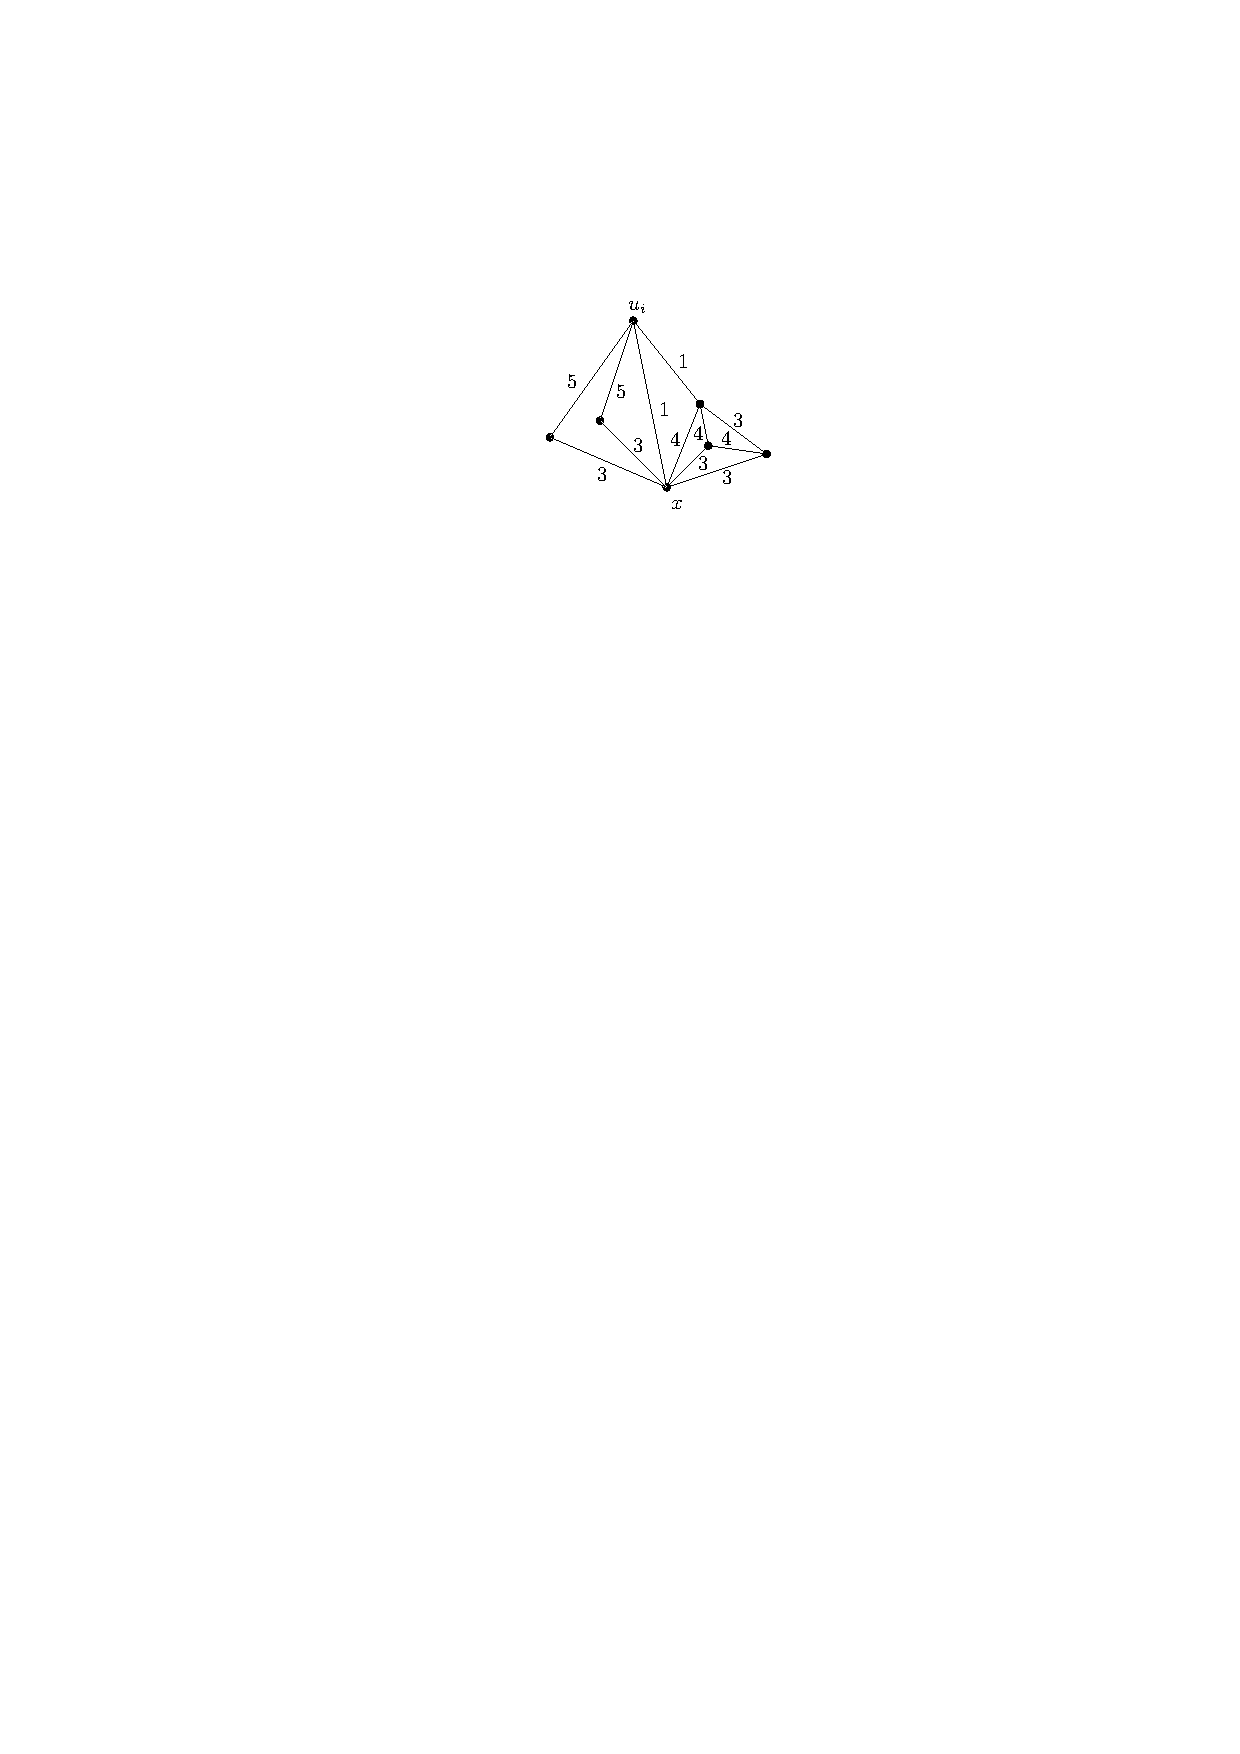
\includegraphics[scale=1.1]{img/act-hamilton-cycle-b}
\caption{The modified version of the type $L$ gadget without edges of weight $7$.}
\label{fig_hamilton_cycle_improved}
\end{figure}
%%%%%%%%%%%%%%%%%%%%%%%%%%

As it is NP-hard to distinguish between {\xxxNTP} instances with optimal objective value~$6$ 
and {\xxxNTP} instances with optimal objective value~$7$, we also get the following 
in approximability result.
%%%%%%%%%%%%%%%%%%%%%%%%%%
\begin{corollary}
\label{coro:inapproximability}
Unless P=NP, there is no polynomial time approximation algorithm for {\xxxNTP} with
worst case guarantee better than $7/6$.
\qed
\end{corollary}
%%%%%%%%%%%%%%%%%%%%%%%%%%


%%%%%%%%%%%%%%%%%%%%%%%%%%%%%%%%%%%%%%%%%%%%%%%%%%%%%%%%%%%%%%%%%%%%%%%%%
%%%%%%%%%%%%%%%%%%%%%%%%%%%%%%%%%%%%%%%%%%%%%%%%%%%%%%%%%%%%%%%%%%%%%%%%%
\section{A Positive Result for Objective Value Three}
\label{sec:value-three}
%%%%%%%%%%%%%%%%%%%%%%%%%%%%%%%%%%%%%%%%%%%%%%%%%%%%%%%%%%%%%%%%%%%%%%%%%
In Section~\ref{sec:value-seven}, we have established the NP-hardness of deciding whether 
there exists a schedule of objective value at least~$7$. 
As a complementary result, we now show that it can be decided in polynomial time whether there is
a schedule of objective value at least~$3$.

%%%%%%%%%%%%%%%%%%%%%%%%%%
\begin{theorem}
\label{th:value=3}
For an instance of {\xxxNTP} on a graph with $m$ edges, it can be decided in $\bigO(m^3)$ time 
whether $\ntp(G,w)\ge3$.
\end{theorem}
%%%%%%%%%%%%%%%%%%%%%%%%%%
\begin{proof}
Let $G=(V,E)$. 
We partition the edge set $E$ into set $W_1$ (edges of weight~$1$), set $W_2$ (edges of weight~$2$),
and set $W_{\ge3}$ (edges of weight at least~$3$).
In a schedule of objective value $3$, we may activate all edges in $W_{\ge3}$ at time~$0$.
We interpret an edge in $W_2$ as a pair of two edges of weight $1$: one of these two edges is scheduled 
during the middle time slot $[1, 2]$; the other edge can either be scheduled during slot $[0,1]$ 
or during slot $[2,3]$. 
Edges in $W_1$ are scheduled during one of the three slots $[0,1]$, $[1,2]$, $[2,3]$.

By Lemma~\ref{le:structure}, we may assume that in a feasible schedule of length~$3$ the 
graphs $(V,E_t)$ with $t=1,2,3$ are trees.
Let $H_3$    be the graph that results from $G$ after contracting the edge set $W_{\ge3}$, and
let $H_{23}$ be the graph that results from $G$ after contracting the edge set $W_2\cup W_{\ge3}$.
We introduce three matroids:
\begin{itemize}
\item The matroid $\mathcal{F}_1$ has the ground set $W_1\cup W_2$. 
A set $F\subseteq W_1\cup W_2$ is independent in $\mathcal{F}_1$, if and only if $F$ is acyclic in graph $H_3$.
\item The matroid $\mathcal{F}_2$ has the ground set $W_1$.
A set $F\subseteq W_1$ is independent in $\mathcal{F}_2$, if and only if $F$ is acyclic in graph $H_{23}$.
\item The matroid $\mathcal{F}_3$ has ground set $W_1\cup W_2$, and coincides with $\mathcal{F}_1$.
\end{itemize}
\lasse{Recall that a base of a matroid is a maximal independent set. By construction, the bases of $\mathcal{F}_1, \mathcal{F}_2$ and $\mathcal{F}_3$ have the following properties. (A small technicality we have to consider is that $W_2$ and $W_{\geq3}$ may contain cycles.)}
\lasse{
\begin{itemize}
\item If a set $F \subseteq W_1 \cup W_2$ is indepenedent in the matroid $\mathcal{F}_1$, then $F$ is a base of $\mathcal{F}_1$ if and only if $F$ induces a spanning tree of $H_3$ if and only if $F \cup W_{\geq 3}$ contains a spanning tree of $G$.
\item If a set $F \subseteq W_1$ is indepenedent in the matroid $\mathcal{F}_2$, then $F$ is a base of $\mathcal{F}_2$ if and only if $F$ induces a spanning tree of $H_{23}$ if and only if $F \cup W_2 \cup W_{\geq 3}$ contains a spanning tree of $G$.
\item If a set $F \subseteq W_1 \cup W_2$ is indepenedent in the matroid $\mathcal{F}_3$, then $F$ is a base of $\mathcal{F}_3$ if and only if $F$ induces a spanning tree of $H_3$ if and only if $F \cup W_{\geq 3}$ contains a spanning tree of $G$.
\end{itemize}
}

\lasse{Now observe that scheduling an edge of weight 1 is equivalent to choosing in which time slot it is scheduled. Scheduling an edge 2 is equivalent to always schedule it in time slot 2 and choose whether it is scheduled in time slot 1 or 3. From these facts we can deduce that we can connect the graph during time slots 1,2 and 3, that is,} $\ntp(G,w)\ge3$ holds, if and only if there exist three pairwise disjoint subsets
$S_1,S_2,S_3$ of $W_1 \cup W_2$, such that $S_t$ forms a base of the matroid $\mathcal{F}_t$ for $t=1,2,3$.
This can be checked in $\bigO(m^3)$ time by using Edmond's matroid partitioning algorithm \cite{edmonds1965minimum}.
\qed
\end{proof}

By a similar (but simpler) argument we can also decide in polynomial time whether $\ntp(G,w)\ge2$.
Deciding whether $\ntp(G,w)\ge1$ is trivial.
The complexity of deciding whether $\ntp(G,w)\ge\beta$ remains open for $\beta\in\{4,5,6\}$.


%%%%%%%%%%%%%%%%%%%%%%%%%%%%%%%%%%%%%%%%%%%%%%%%%%%%%%%%%%%%%%%%%%%%%%%%%
%%%%%%%%%%%%%%%%%%%%%%%%%%%%%%%%%%%%%%%%%%%%%%%%%%%%%%%%%%%%%%%%%%%%%%%%%
\section{The Greedy Algorithm}
\label{sec:greedy}
%%%%%%%%%%%%%%%%%%%%%%%%%%%%%%%%%%%%%%%%%%%%%%%%%%%%%%%%%%%%%%%%%%%%%%%%
We introduce a greedy algorithm that maintains connectivity by always
activating edges of the largest possible weight.
Formally, we let $F_t\subseteq E_t$ denote the set of edges whose activity intervals 
end at time $t$.
By $U_t=E-(E_1\cup E_2\cup\cdots\cup E_t)$ we denote the set of edges that have not been 
used and activated before time $t$.

Now the {\greedy} algorithm starts its work by initializing 
$E_0:=\emptyset$, $F_0:=\emptyset$, and $U_0:=E$.
For $t\ge0$, the set $E_{t+1}$ for time slot $[t,t+1]$ is computed as follows.
If the graph $(V,E_t-F_t)$ is a tree, we set $E_{t+1}:=E_t$.
If the graph $(V,E_t-F_t)$ is a forest with $c$ components, we turn it into 
a tree by adding a maximum weight subset $A\subseteq U_t$ of cardinality $c-1$;
then we set $E_{t+1}:=(E_t-F_t)\cup A$.
In case no such set $A$ exists, the {\greedy} algorithm terminates.
(The set $A$ can be computed for instance by applying Kruskal's algorithm for 
maximum spanning trees; ties are broken arbitrarily.)

%%%%%%%%%%%%%%%%%
\begin{theorem}
\label{th:greedy.approx}
For every graph $G=(V,E)$ on $n$ vertices and for every $w:E\to\NN_0$, 
the {\greedy} algorithm computes a schedule of length at least $\ntp(G,w)/(n-1)$.
Furthermore, there exist instances on which the schedule computed by the 
{\greedy} algorithm is a factor $\lfloor n/2\rfloor$ below the optimal objective value.
\end{theorem}
%%%%%%%%%%%%%%%%%
\begin{proof}
For the positive result, we consider the time slot $[T,T+1]$ at which {\greedy} terminates.
Then the graph $(V,(E_T-F_T)\cup U_T)$ is not connected.
We consider the vertex set $C\subseteq V$ of one of the components of that graph, and the
corresponding edge cut $\delta(C)$.
Then the weight $w(\delta(C))=\sum_{e\in\delta(C)}w(e)$ yields a trivial upper bound for the 
optimal objective value: 
%%%%%%%%%%%%%%%%%
\begin{equation}
\label{eq:greedy}
\ntp(G,w) ~\le~ w(\delta(C))
\end{equation}
%%%%%%%%%%%%%%%%%
Since every edge set $E_j$ with $1\le j\le T$ induces a tree, we have $|E_j|=n-1$ and hence
$|E_j\cap \delta(C)|\le n-1$.
As all edges in the cut $\delta(C)$ have been activated and run to completion before the 
time slot $[T,T+1]$, we conclude $T\ge w(\delta(C))/(n-1)$, which together with \eqref{eq:greedy}
yields the desired approximation guarantee.

For the negative result, we consider the complete graph $K_n=(V,E)$ on $n$ vertices with 
weights $w(e)=1$ for all $e\in E$.
A folklore result (see for instance Palmer~\cite{Palmer2001}) says that the maximum number of 
edge-disjoint spanning trees that can be packed into $K_n$ is $\lfloor n/2\rfloor$.
This implies $\ntp(K_n,w)=\lfloor n/2\rfloor$.
On the other hand, if the {\greedy} algorithm at time $0$ activates the $n-1$ edges in the edge
cut $\delta(v)$ for some $v\in V$, the objective value of the resulting schedule equals~$1$.
\qed
\end{proof}


%%%%%%%%%%%%%%%%%
\begin{theorem}
\label{th:greedy.cactus}
For every connected graph $G=(V,E)$, the following two statements are equivalent.
\begin{enumerate}[(i)]
\item $G$ is a cactus graph.
\item For every choice $w:E\to\NN_0$ of edge weights, the {\greedy} algorithm 
solves the {\xxxNTP} instance $(G,w)$ to optimality.
\end{enumerate}
\end{theorem}
%%%%%%%%%%%%%%%%%
%%%%%%%%%%%%%%%%%%%%%%%%%%%%%%%%%%%%%%%%%
\begin{figure}[tbh]
\begin{center}
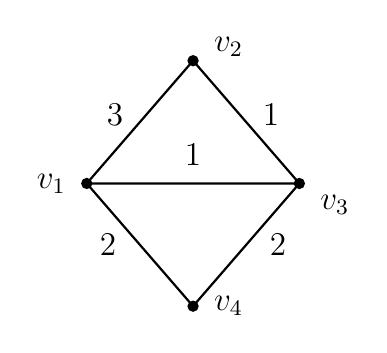
\begin{tikzpicture}[scale=0.90]

\coordinate (p1) at (-1.5, 0.000);
\coordinate (p2) at ( 0.0, 1.732);
\coordinate (p3) at ( 1.5, 0.000);
\coordinate (p4) at ( 0.0,-1.732);
\foreach \x in {1,...,4}{\fill (p\x) circle (0.08);}

\node at ($(p1)+(-0.5, 0.00)$) {\large $v_1$};
\node at ($(p2)+(+0.5, 0.20)$) {\large $v_2$};
\node at ($(p3)+(+0.5,-0.30)$) {\large $v_3$};
\node at ($(p4)+(+0.5, 0.00)$) {\large $v_4$};

\draw[thick] (p1)--(p2)--(p3)--(p4)--(p1)--(p3);
\node at ($(p1)!0.5!(p2)+(-0.35, 0.1)$) {\large $3$};
\node at ($(p1)!0.5!(p4)+(-0.45, 0.0)$) {\large $2$};
\node at ($(p1)!0.5!(p3)+( 0.00, 0.4)$) {\large $1$};
\node at ($(p2)!0.5!(p3)+(+0.35, 0.1)$) {\large $1$};
\node at ($(p4)!0.5!(p3)+(+0.45, 0.0)$) {\large $2$};
\end{tikzpicture}
\end{center}
\caption{An instance $(H,w_H)$ on which the {\greedy} algorithm fails.}
\label{fig:cactus}
\end{figure}
%%%%%%%%%%%%%%%%%%%%%%%%%%%%%%%%%%%%%%%%%
\begin{proof}
We first show that (i) implies (ii).
Since cut-vertices split an {\xxxNTP} instance into smaller instances that do not interact 
with each other, it is sufficient to prove the statement for two-connected cactus graphs.
Hence we will assume that $G$ is a cycle on $n$ vertices, and we let $e_1,\ldots,e_n$ 
denote the edges in the cycle ordered by increasing weight so that 
$w(e_1)\le w(e_2)\le\cdots\le w(e_n)$.
It is easily seen that the optimal objective value for $(G,w)$ equals 
$\min\{w(e_1)+w(e_2),\,w(e_3)\}$.
As the {\greedy} algorithm activates the $n-1$ edges $e_2,\ldots,e_n$ at time~$0$ and 
activates the final edge $e_1$ at time $w(e_2)$, it yields the optimal objective value.

In order to show that (ii) implies (i), we first consider the graph $H$ on the four
vertices $v_1,v_2,v_3,v_4$ and the edge weights $w_H$ depicted in Figure~\ref{fig:cactus}.
As the {\greedy} algorithm at time~$0$ activates the three edges $\{v_1,v_2\}$, $\{v_1,v_4\}$, 
$\{v_3,v_4\}$ (that carry the weights $3,2,2$, respectively), at time~$2$ there remains no 
further possibility of connecting vertex $v_4$ to the rest of the graph; hence {\greedy} 
generates a schedule of value~$2$.
On the other hand, the optimal schedule results by activating the three edges $\{v_1,v_2\}$, 
$\{v_1,v_3\}$, $\{v_3,v_4\}$ at time~$0$, by activating edge $\{v_1,v_4\}$ at time~$1$,
and by activating edge $\{v_2,v_3\}$ at time~$2$; the corresponding optimal objective
value is $\ntp(H,w_H)=3$.
Hence {\greedy} fails to solve this instance $(H,w_H)$ to optimality.

Now let $G=(V,E)$ be an arbitrary connected graph that is not a cactus. 
This implies that $G$ does contain a subdivision $(V',E')$ of the four-vertex 
graph $H=(V_H,E_H)$ in Figure~\ref{fig:cactus}.
Let $E''\subseteq E$ be a subset of cardinality $|V-V'|$, so that the graph $(V,E'\cup E'')$
is connected.
We construct edge weights $w:E\to\NN_0$ as follows.
For every edge $e\notin E'\cup E''$ we set $w(e)=0$, and
for every edge $e\in E''$ we set $w(e)=3$.
Finally, we fix the weights $w(e)$ of the edges $e\in E'$ so that they emulate the 
weights $w_H:E_H\to\NN_0$ in the four-vertex graph $H$; if an edge $e\in E'$ belongs to the 
subdivision of some edge $f\in E_H$, we define $w(e)=w_H(f)$.
It is easily verified that the resulting instance $(G,w)$ satisfies $\ntp(G,w)=3$,
whereas the {\greedy} algorithm only yields an objective value of~$2$.
\qed
\end{proof}


%%%%%%%%%%%%%%%%%%%%%%%%%%%%%%%%%%%%%%%%%%%%%%%%%%%%%%%%%%%%%%%%%%%%%%%%%
%%%%%%%%%%%%%%%%%%%%%%%%%%%%%%%%%%%%%%%%%%%%%%%%%%%%%%%%%%%%%%%%%%%%%%%%%
\section{Parameterized Complexity}
\label{sec:parameterized}
%%%%%%%%%%%%%%%%%%%%%%%%%%%%%%%%%%%%%%%%%%%%%%%%%%%%%%%%%%%%%%%%%%%%%%%%%
In this section, we show that problem {\xxxNTP} is fixed parameter tractable with 
respect to various parameters. 
Note that Theorems~\ref{thm:hardness_complete_bipartite} and \ref{th:value=7} imply the NP-hardness 
of problem {\xxxNTP}, even if either the treewidth or the edge weights are bounded by a constant. 

\begin{restatable}{theorem}{fptBoundedWeightAndTW}
\label{th:fpt_weights_and_tw_bounded}
If both the treewidth and the maximum edge weight of the input graph $G = (V, E)$ are bounded, problem {\xxxNTP} allows for an FPT-algorithm whose running time is linear in $|E|$. 
\end{restatable}
\begin{proof}
As the graph $G=(V,E)$ has treewidth at most $k$, there is a vertex $v\in V$ of degree at most $k$ \lasse{(note that we use here the property that $G$ is a simple graph, that is, it has no parallel edges.)}.
As every edge incident to $v$ has weight at most $k$, we conclude $\ntp(G,w)\le k^2$. 
For every $T=1,\ldots,k^2$, we construct a formula $\Phi_T$ in monadic second-order 
graph logic $\text{MSO}_2$, so that $\Phi_T$ is satisfiable if and only if there exists a schedule 
of objective value at least $T$. 
We introduce Boolean variables $x_{e,t}$ for every $e\in E$ and every $t\in \{1,\dots,T\}$
to denote whether $e\in E_t$. 
The following statement can be formulated in $\text{MSO}_2$ by routine methods:
\begin{align*}
\exists \sigma: E\to\{0,\ldots,&T\} ~~\forall e\in E ~~\forall t\in\{1,\ldots,T\}: \\
& x_{e,t} \iff \left(\sigma(e) < t \leq \sigma(e) + w(e)\right)\\
& \land \forall t\in\{1,\ldots,T\}: \set{e\in E \mid x_{e,t}} \text{ is a spanning tree.}
\end{align*}
Now Courcelle's theorem \cite{courcelle1990monadic} implies that the satisfiability of $\Phi_T$ 
can be checked in linear time for every $T=1,\ldots,k^2$.
\qed
\end{proof}

\begin{restatable}{theorem}{exactAlgoExponential}
\label{th:exact}
On input graphs $G=(V,E)$, problem {\xxxNTP} is solvable in exponential time $\bigO(|E|^2\cdot|E|!)$. 
\end{restatable}
\begin{proof}
By Lemma~\ref{le:structure}, we may assume that in an optimal schedule $\sigma$ of length $T$ 
all graphs $G_1^\sigma, \dots, G_T^\sigma$ are trees.
As these trees are uniquely determined by the ordering in which $\sigma$ activates the edges,
we only need to check and evaluate $|E|!$ cases.
Each case is easily checked and evaluated in $\bigO(|E|^2)$ time.
\qed
\end{proof}

\begin{restatable}{theorem}{fptFeedbackEdge}
\label{thm:FPT_feedback_edge_set}
Problem {\xxxNTP} is fixed parameter tractable with respect to the size $k$ of a feedback edge set. 
There is a kernel with $\bigO(k)$ vertices and edges. 
\end{restatable}
\begin{proof}
Note that the input graph $G=(V,E)$ satisfies $|E|\le|V|-1+k$.
We first prove an auxiliary observation on the largest edge weight $w_{\max}$ in the graph:
We claim that $|V|\ge k+2$ implies $\ntp(G,w)\le w_{\max}$. 
Consider an optimal schedule as in Lemma~\ref{le:structure}, so that $|E_1|=|V|-1$.
As every edge in $E_1$ is certainly inactive from time $w_{\max}$ onwards, there remain at most 
$|E|-|E_1|=|E|-|V|+1\le k$ edges that could become active during the next time slot $[w_{\max},w_{\max}+1]$.
As a spanning tree needs at least $|V|-1\ge k+1$ edges, this proves the auxiliary observation.
As a consequence we get that in an optimal schedule an edge with weight $w_{\max}$ without loss 
of generality may be activated at time~$0$.

Now the kernelization procedure is clear:
As long as $|V|\ge k+2$ holds, we contract an edge with largest edge weight.
Note that the contraction maintains the inequality $|E|\le|V|-1+k$.
The resulting kernel satisfies $|V|\le k+1$ and $|E|\le2k$.
\qed
\end{proof}


The last theorem of this section shows that problem {\xxxNTP} is tractable on instances that in 
a certain sense are close to the preemptive tree packing problem \eqref{eq:NW.1}--\eqref{eq:NW.3}. 
%%%%%%%%%%%%%%%%%%
\begin{restatable}{theorem}{fptAlmostAllWeightOne}
\label{th:fpt_almost_all_weight_one}
Let $(G,w)$ be an instance of {\xxxNTP} on $m$ edges, so that $m-k$ edges have weight~$1$ and 
the remaining $k$ edges have weight at most $k$. 
Then an optimal solution can be found in $\bigO(k^{2k}m^3)$ time.
\end{restatable}
%%%%%%%%%%%%%%%%%%
\begin{proof}
Let $E'=\set{e\in E: w(e)\ne1}$. 
For a schedule $\sigma$ of objective value $T$, we denote by $D_\sigma= \set{t: E_t^\sigma\cap E'\ne\emptyset}$ 
the set of time slots $[t-1,t]$ during which at least one edge of $E'$ is active. 
For every $t\le T$ with $t\notin D_\sigma$, graph $G_t=(V,E_t)$ is a connected graph in which 
all edges have weight 1.  
For each such $t$ with $t \not\in D_\sigma$, we introduce another schedule $\pi$, where the edge set $E_t$ is scheduled in the last time 
slot $[T-1, T]$ instead of the $t$-th time slot, and all edges activated during $[t, T]$ are activated 
one time unit earlier instead. Formally, schedule $\pi$ is such that
%%%%%%%%%%%%%%%%%%
\[(G^\pi_1,\dots, G^\pi_T) = (G^\sigma_1, \dots G^\sigma_{t-1}, G^\sigma_{t+1}, \dots, G^\sigma_T, G^\sigma_t). \]
%%%%%%%%%%%%%%%%%%
Observe that $\pi$ is also a schedule of objective value $T$. 
By repeating this procedure often enough, we conclude that there always exists an optimal schedule $\sigma$ so that $D_\sigma \subseteq \fromto{1}{k^2}$. 
Due to \cref{le:structure}, we can additionally require that each of $G_1, \dots, G_T$ is acyclic.

Therefore, the following is an algorithm to solve problem {\xxxNTP}: 
Iterate over all possible $k^{2k}$ choices of $(\sigma(e))_{e \in E'} \in \fromto{1}{k^2}^k$. 
For each fixed choice, the only edges left to schedule are edges of weight one. 
This can be done optimally the following way: 
For $t = 1,\dots, k^2$, let $W_t = \set{e \in E' : \sigma(e) < t \leq \sigma(e) + w(e)}$ be the set of edges in $E'$, which are active during the $t$-th time slot. 
If some $W_t$ has a cycle, we immediately skip to the next choice of $(\sigma(e))_{e \in E'}$. 
Otherwise, consider the matroid $\mathcal{F}_t = \set{F \subseteq E(G)-E' : W_t \cup F \text{ is acyclic}}$. 
We extend the definition of $\mathcal{F}_t$ to $t > k^2$ by setting $W_t = \emptyset$ in this case. 
The matroid $\mathcal{F}_t$ is isomorphic to the graphic matroid of $G$ after contracting each connected 
component of $W_t$ to a single vertex. 
Now we run Edmond's Matroid Partitioning algorithm \cite{edmonds1965minimum} to determine the 
maximal $T'\in\NN_0$ such that $E(G)-E'$ contains disjoint sets $F_1, \dots, F_{T'}$ such that $F_t$ 
is a base of $\mathcal{F}_t$ for all $t \in \fromto{1}{T'}$ (that is, we solve the problem of packing as 
many bases as possible into a matroid). 
As Edmond's Matroid Partitioning algorithm runs in $\bigO(m^3)$ time, the claimed time complexity follows.
\qed
\end{proof}


%%%%%%%%%%%%%%%%%%%%%%%%%%%%%%%%%%%%%%%%%%%%%%%%%%%%%%%%%%%%%%%%%%%%%%%%%
%%%%%%%%%%%%%%%%%%%%%%%%%%%%%%%%%%%%%%%%%%%%%%%%%%%%%%%%%%%%%%%%%%%%%%%%%


%%%%%%%%%%%%%%%%%%%%%%%%%%%%%%%%%%%%%%%%%%%%%%%%%%%%%%%%%%%%%%%%%%%%%%%%%
%%%%%%%%%%%%%%%%%%%%%%%%%%%%%%%%%%%%%%%%%%%%%%%%%%%%%%%%%%%%%%%%%%%%%%%%%
\section{Conclusion}
\label{sec:conclusion}
%%%%%%%%%%%%%%%%%%%%%%%%%%%%%%%%%%%%%%%%%%%%%%%%%%%%%%%%%%%%%%%%%%%%%%%%%
We have analyzed the computational complexity and the algorithmic behavior of non-preemptive
tree packing.
The problem is strongly NP-hard even on highly structured and extremely simple graph classes,
and we only have a handful of positive results.

There remain many open questions.
~(Q1) We have shown that {\xxxNTP} can be approximated in polynomial time within a factor of $n-1$, 
and that no approximation factor better than $7/6$ is possible (unless P=NP).
Where is the true approximation threshold?
In particular, we would like to know whether our problem allows a polynomial time approximation
algorithm with some constant worst case guarantee.
A major step towards an answer might be the analysis of the gap between the non-preemptive optimum 
and the polynomially computable preemptive optimum for problem \eqref{eq:NW.1}--\eqref{eq:NW.3}.
~(Q2) If all edge weights are equal to~$1$, problem {\xxxNTP} coincides with the preemptive problem 
version and hence is polynomially solvable.
On the other hand the problem is NP-hard, if all edge weights are in $\fromto{1}{6}$. 
What is the complexity of {\xxxNTP}, if all edge weights are in $\{1,2\}$?
~(Q3) The problem of deciding whether $\ntp(G,w)\ge\beta$ is polynomially solvable for 
every $\beta\le3$ and NP-hard for every $\beta\ge7$.
What is the complexity of this question for $\beta\in\{4,5,6\}$?


%%%%%%%%%%%%%%%%%%%%%%%%%%%%%%%%%%%%%%%%%%%%%%%%%%%%%%%%%%%%%%%%%%%%%%%%%
%%%%%%%%%%%%%%%%%%%%%%%%%%%%%%%%%%%%%%%%%%%%%%%%%%%%%%%%%%%%%%%%%%%%%%%%%
\subsubsection*{Acknowledgements.}
Stefan Lendl and Lasse Wulf acknowledge the support of the Austrian Science Fund (FWF): W1230.
Gerhard Woeginger acknowledges support by the DFG RTG 2236 ``UnRAVeL''.

%
% ---- Bibliography ----
%
% BibTeX users should specify bibliography style 'splncs04'.
% References will then be sorted and formatted in the correct style.


%%%%%%%%%%%%%%%%%%%%%%%%%%%%%%%%%%%%%%%%%%%%%%%%%%%%%%%%%%%%%%%%%%%%%%%%%
%%%%%%%%%%%%%%%%%%%%%%%%%%%%%%%%%%%%%%%%%%%%%%%%%%%%%%%%%%%%%%%%%%%%%%%%%
\bibliographystyle{splncs04}
\bibliography{literature}

%%%%%%%%%%%%%%%%%%%%%%%%%%%%%%%%%%%%%%%%%%%%%%%%%%%%%%%%%%%%%%%%%%%%%%%%%
%%%%%%%%%%%%%%%%%%%%%%%%%%%%%%%%%%%%%%%%%%%%%%%%%%%%%%%%%%%%%%%%%%%%%%%%%





\end{document}
